% This file was converted to LaTeX by Writer2LaTeX ver. 1.0.2
% see http://writer2latex.sourceforge.net for more info
\documentclass[a4paper,11pt]{article}
\usepackage[ascii]{inputenc}
\usepackage[T1]{fontenc}
\usepackage[italian]{babel}
\usepackage{amsmath}
\usepackage{amssymb,amsfonts,textcomp}
\usepackage{color}
\usepackage{array}
\usepackage[square,numbers]{natbib}
\usepackage{url}
\usepackage{supertabular}
\usepackage{hhline}
\usepackage{hyperref}
\hypersetup{pdftex, colorlinks=true, linkcolor=blue, citecolor=black, filecolor=blue, urlcolor=blue, pdftitle=, pdfauthor=, pdfsubject=, pdfkeywords=}
\usepackage[pdftex]{graphicx}
% Outline numbering
\setcounter{secnumdepth}{0}
\makeatletter
\newcommand\arraybslash{\let\\\@arraycr}
\makeatother
% Page layout (geometry)
\setlength\voffset{-1in}
\setlength\hoffset{-1in}
\setlength\topmargin{2cm}
\setlength\oddsidemargin{2cm}
\setlength\textheight{24.777668cm}
\setlength\textwidth{17.001cm}
\setlength\footskip{26.144882pt}
\setlength\headheight{0cm}
\setlength\headsep{0cm}
% Footnote rule
\setlength{\skip\footins}{0.119cm}
\renewcommand\footnoterule{\vspace*{-0.018cm}\setlength\leftskip{0pt}\setlength\rightskip{0pt plus 1fil}\noindent\textcolor{black}{\rule{0.25\columnwidth}{0.018cm}}\vspace*{0.101cm}}
% Pages styles
\makeatletter
\newcommand\ps@Standard{
  \renewcommand\@oddhead{}
  \renewcommand\@evenhead{}
  \renewcommand\@oddfoot{\thepage{}}
  \renewcommand\@evenfoot{\@oddfoot}
  \renewcommand\thepage{\arabic{page}}
}
\makeatother
\pagestyle{Standard}
\setlength\tabcolsep{1mm}
\renewcommand\arraystretch{1.3}
% footnotes configuration
\makeatletter
\renewcommand\thefootnote{\arabic{footnote}}
\makeatother
% Non-floating captions
\makeatletter
\newcommand\captionof[1]{\def\@captype{#1}\caption}
\makeatother
\date{2011-06-30}

\title{Sviluppo di server web e sistema di caching per contenuti dinamici}
\author{Salvatore Tomaselli}

\begin{document}

\begin{titlepage}
\begin{center}

\textsc{\LARGE UNIVERSIT\`{A} DEGLI STUDI DI CATANIA}\\[0.5cm]

\textsc{\Large Facolt\`{a} di Scienze Matematiche Fisiche e Naturali}\\[0.5cm]
\textsc{\Large Corso di Laurea in Informatica}\\[0.5cm]


\line(1,0){250}


{ \huge \bfseries Sviluppo di server web e sistema di caching per contenuti dinamici}\\[0.4cm]

\begin{minipage}{0.4\textwidth}
\begin{flushleft} \large
\emph{Autore:}\\
Salvatore \textsc{Tomaselli}
\end{flushleft}
\end{minipage}
\begin{minipage}{0.4\textwidth}
\begin{flushright} \large
\emph{Relatore:} \\
Prof.~Giuseppe \textsc{Pappalardo}
\end{flushright}
\end{minipage}

\vfill
\line(1,0){250}

{\large 2011-06-30}



\end{center}
\end{titlepage}

\section{Abstract}
Sharing a large amount of files on GNU/Linux and other Unix systems can be a complex operation:
most solutions require installing and configuring some kind of file server that requires root permissions to run correctly. Other solutions are emails or physical supports.

This thesis describes Weborf, a project to implement a HTTP server as a viable solution for filesharing without root permissions.

Being aimed also at low end/embedded devices, a caching mechanism for content generated by the server itself is imlpemented and solutions to retrieve the cache items, invalidate them, deal with concurrency are shown.

\setcounter{tocdepth}{10}
\renewcommand\contentsname{Indice}
\tableofcontents
\listoffigures
\listoftables
\section{Introduzione}
{\sffamily
Condividere grosse quantit\`a di file su GNU/Linux e su altri sistemi
Unix pu\`o essere una operazione complicata per gli utenti.}

{\sffamily
Le soluzioni pi\`u note riguardano l{\textquotesingle}utilizzo si FTP,
SAMBA o NFS. Tuttavia queste soluzioni richiedono i permessi di super
utente (per avviare il server o montare il filesystem), quindi \`e
necessario l{\textquotesingle}intervento di un amministratore di
sistema. Anche SSH pu\`o venir utilizzato a tal scopo, ma anche esso
presenta gli stessi problemi.}

{\sffamily
Altre soluzioni sono naturalmente disponibili per gli utenti, come
l{\textquotesingle}invio di email o la copia dei file utilizzando
supporti fisici. Anche l{\textquotesingle}invio tramite una linea di
comando simile alla seguente:}

{\ttfamily
tar -c directory/ {\textbar} nc destination 5005}

{\sffamily
\`e possibile, ma di certo poco agevole.}


\bigskip

{\sffamily
Il progetto nasce quindi con l{\textquotesingle}intenzione di
semplificare la condivisione di file e intere directory sulla rete,
anche per utenti senza privilegi di root e con conoscenze dei sistemi
Unix non necessariamente molto vaste.}


\bigskip

{\sffamily
Si osserva che il protocollo HTTP \`e tra i pi\`u utilizzati in
assoluto, e che dispone di una ampia variet\`a di client e di server su
tutti i sistemi operativi. Ne consegue che la maggior parte degli
utenti di qualsiasi piattaforma sono abituati
all{\textquotesingle}utilizzo di client HTTP e che
l{\textquotesingle}operazione di download di un file non pone
solitamente alcuna difficolt\`a.}


\bigskip

\section{Analisi requisiti - specifiche}
{\sffamily
Il software deve implementare un web-server con alcune caratteristiche
che lo rendano utilizzabile da diverse categorie di utenti, con
specifiche necessit\`a.}


\bigskip

{\sffamily
Il software dovr\`a essere compatibile allo standard POSIX, e ci si
riferir\`a ad {\textquotedbl}Open Group{\textquotedbl} per verificare
che non vengano utilizzate caratteristiche specifiche di una
piattaforma piuttosto che un{\textquotesingle}altra. La stretta
attinenza allo standard POSIX deve permettere al software di funzionare
sulle piattaforme che implementano tale standard, ottenendo quindi una
compatibilit\`a a livello di codice sorgente ma non quella binaria.}

{\sffamily
Durante lo sviluppo sar\`a necessario tenere conto del fatto che il
sistema Mac OsX implementa la versione 2001 dello standard ma non le
successive\cite{MAC01}, quindi per ottenere la portabilit\`a su tale sistema
potrebbe essere necessario evitare di utilizzare nuove caratteristiche.
}


\bigskip

{\sffamily
Per maggiore compatibilit\`a, il software dovr\`a essere capace di
utilizzare il protocollo di rete IPv6, senza tuttavia precludere la
possibilit\`a di essere eseguito su piattaforme che supportano
unicamente il protocollo IPv4.}


\bigskip

{\sffamily
\`E consigliabile progettare la struttura in modo che sia possibile
attivare o disattivare funzionalit\`a in fase di compilazione.}


\bigskip

{\sffamily
La prima categoria di utenti a cui il software si rivolge, \`e quella
degli utenti desktop che desiderano condividere dei file o intere
directory in rete.}

{\sffamily
Non viene fatta l{\textquotesingle}assunzione che tali utenti possano
elevare i propri privilegi a piacimento. Deve quindi essere possibile
eseguire il software senza privilegi di root.}

{\sffamily
Dato che l{\textquotesingle}utente potrebbe voler condividere dei file
con estensione .php o altri file eseguibili, deve essere possibile
disattivare il supporto al protocollo CGI.}

{\sffamily
Un utente potrebbe voler condividere diverse directory di volta in
volta, quindi il software deve essere in grado di accettare come
parametro la directory da condividere.}

{\sffamily
Quando il client dovesse richiedere un URL corrispondente ad una
directory, il server dovr\`a verificare la presenza di un file index
all{\textquotesingle}interno della stessa, e in sua mancanza dovr\`a
generare dinamicamente una pagina HTML con l{\textquotesingle}elenco di
file contenuti, link agli stessi ed eventualmente vari dettagli.
Inoltre se la directory non \`e quella di base, dovr\`a essere presente
un link alla directory superiore (..).}

{\sffamily
Per gli utenti che volessero condividere intere directory sotto forma di
file .tar, una opzione deve consentire tale modalit\`a.}

{\sffamily
Per questa categoria di utenti, \`e preferibile che il software possa
funzionare senza nessun file di configurazione, ma utilizzando soltanto
uno o due parametri al massimo sulla linea di comando.}

{\sffamily
Dato che per utilizzare la porta 80 di default per il protocollo HTTP
sono necessari i privilegi di super utente, il software dovr\`a
utilizzare la porta 8080 come default (definita come http-alt)\cite{STD04},
se non diversamente specificato al momento
dell{\textquotesingle}esecuzione.}

{\sffamily
Per semplificare l{\textquotesingle}utilizzo da parte degli utenti, deve
essere disponibile una interfaccia grafica che consenta un rapido
utilizzo del software senza necessit\`a di avere una elevata
comprensione del sistema.}

{\sffamily
Tale interfaccia grafica dovr\`a consentire agli utenti di scegliere
quale directory intendono condividere, specificare le impostazioni di
rete ed eventuali modifiche ai permessi di accesso di default. Inoltre
una volta attivata la condivisione dovr\`a fornire
all{\textquotesingle}utente un rapido accesso all{\textquotesingle}URL
corrispondente ai file condivisi.}


\bigskip

{\sffamily
La seconda categoria di utenti considerata, comprende gli sviluppatori
web o gli amministratori di sistema che necessitano di un server web di
prova.}

{\sffamily
Questi utenti potrebbero avere la possibilit\`a di elevare i propri
privilegi, ma anche in questo caso la possibilit\`a di eseguire il
software senza privilegi di root deve essere garantita, per maggiore
sicurezza.}

{\sffamily
Il software deve implementare il protocollo CGI come definito dalla RFC
3875, con speciale riguardo verso l{\textquotesingle}esecuzione di
programmi in PHP.}

{\sffamily
Per evitare programmi CGI che non terminano ed occupano le risorse in
modo indefinito, il server deve tentare di chiudere il programma dopo
un timeout.}


\bigskip

{\sffamily
La terza categoria di utenti riguarda quelli che intendono utilizzare
weborf come server di produzione.}

{\sffamily
Per essere utilizzato da tale categoria, il software deve fornire la
possibilit\`a di essere avviato da super utente dal processo init,
questa modalit\`a di utilizzo verr\`a chiamata
{\textquotedbl}demone{\textquotedbl}.}

{\sffamily
In questa modalit\`a il software dovr\`a acquisire la porta TCP e
ridurre i propri privilegi immediatamente dopo.}

{\sffamily
In modalit\`a demone il software dovr\`a utilizzare un file di
configurazione opportunamente documentato da un file di manuale.
Inoltre si dovr\`a distribuire un file di configurazione di esempio ma
gi\`a funzionante, in modo da rendere il server pronto immediatamente
dopo l{\textquotesingle}installazione.}

{\sffamily
Tale file di configurazione dovr\`a fornire un elenco ordinato di
possibili nomi per i file index che bloccano il listing della
directory, dovr\`a indicare la directory di partenza utilizzata.
Inoltre dovr\`a indicare l{\textquotesingle}utente che verr\`a
utilizzato dopo aver acquisito la porta 80, e dovr\`a anche specificare
se il CGI \`e attivo o meno.}

{\sffamily
Il software deve anche fornire la capacit\`a di utilizzare i virtual
host (come definita nella RFC 2616), e quindi servire
contemporaneamente diversi domini. I differenti domini dovranno essere
inseriti nel file di configurazione.}

{\sffamily
Lo script di avvio per la modalit\`a demone dovr\`a accettare i consueti
parametri {\textquotedbl}start{\textquotedbl}
{\textquotedbl}stop{\textquotedbl}
{\textquotedbl}restart{\textquotedbl}
{\textquotedbl}status{\textquotedbl}, ma dovr\`a anche essere
compatibile con Linux Standard Base (LSB).}

{\sffamily
Weborf dovr\`a anche registrare l{\textquotesingle}attivit\`a nei log di
sistema, utilizzando il demone syslog.}

{\sffamily
Deve anche fornire autenticazione Basic, come definita dalla RFC 2617.
Per ottenere una maggiore flessibilit\`a
nell{\textquotesingle}autenticazione, la decisione di garantire una
richiesta o meno deve essere presa da un processo esterno che non \`e
parte del progetto ma dovr\`a essere scritto in base alle esigenze
specifiche.}

{\sffamily
Per un utilizzo in produzione, weborf deve essere in grado di scalare in
base al traffico, di poter rimanere in esecuzione ininterrotta per un
periodo di tempo indefinito senza presentare memory leak che ne
renderebbero necessario il riavvio. Inoltre deve essere resistente a
richieste appositamente malformate.}

{\sffamily
Per l{\textquotesingle}utilizzo in ambienti di produzione con poche
risorse (come sistemi embedded) il server deve poter funzionare tramite
il demone xinetd.}


\bigskip

{\sffamily
Il server deve anche implementare i metodi HTTP definiti
nell{\textquotesingle}ultima versione del protocollo PUT e DELETE. Dato
che questi metodi offrono la possibilit\`a di modifica di file
residenti sul server, l{\textquotesingle}uso di questi metodi deve
essere disabilitato di default e consentito soltanto nel caso in cui
venga utilizzata l{\textquotesingle}autenticazione. In tale caso si
potr\`a assumere che le richieste autorizzate siano quelle valide e
quindi tali metodi potranno essere attivati.}

{\sffamily
Inoltre il server deve fornire una implementazione parziale del
protocollo webdav definito nella RFC 2518, tale implementazione deve
essere sufficiente a montare le directory usando i client dav di KDE,
Gnome, davfs.}

{\sffamily
Devono essere implementati i metodi webdav: PROPFIND, MOVE, COPY, MKCOL.
Anche tali metodi devono essere utilizzabili solo nel caso
l{\textquotesingle}autenticazione sia in uso.}


\bigskip

\section{Linguaggio e tool}
{\sffamily
Viene utilizzato per lo sviluppo del server il linguaggio C, nella
versione C99.}

{\sffamily
Per la compilazione e la distribuzione vengono usati i GNU Autotools,
che consentono di verificare la presenza delle librerie necessarie, e
di aggiungere le necessarie macro al codice per reagire di conseguenza
alla presenza o all{\textquotesingle}assenza di certe librerie, o alla
differente dimensione dei tipi di dati su sistemi e architetture
differenti.}


\bigskip

{\sffamily
Alcune delle importanti funzioni fornite da GNU Autoconfig \`e la
rilevazione di librerie che potrebbero non essere presenti su tutti i
sistemi su cui si desidera compilare, l{\textquotesingle}assenza di
alcune librerie causa la compilazione di weborf senza la presenza del
supporto per la caratteristica\cite{GNU01}. Autoconfig consente anche la
compilazione di codice in grado di gestire i file grandi su tutte le
architetture.}

{\sffamily
Nel caso di funzioni indispensabili (come la libreria pthread),
Autoconfig \`e configurato per causare il fallimento dello script di
configurazione.}


\bigskip

{\sffamily
Il compilatore preferito per lo sviluppo \`e GNU Compiler Collection
GCC-4.6.}

{\sffamily
Per l{\textquotesingle}individuazione di memory leaks e in generale
errori nell{\textquotesingle}uso della memoria, vengono usati gdb e
valgrind.}


\bigskip

{\sffamily
La linea di comando di valgrind utilizzata \`e la seguente:}

{\ttfamily
valgrind -v -{}-track-origins=yes -{}-tool=memcheck -{}-leak-check=yes
-{}-leak-resolution=high -{}-show-reachable=yes -{}-num-callers=20
-{}-track-fds=yes ./weborf}

{\sffamily
ed \`e consigliabile che l{\textquotesingle}eseguibile abbia ancora i
simboli di debug}


\bigskip

{\sffamily
Inoltre per fare analisi statica del codice \`e stata utilizzata la
suite Clang/LLVM \`e stato usato il seguente comando con i seguenti
parametri:}

{\ttfamily
scan-build gcc -c *.}


\bigskip

{\sffamily
scan-build individua problemi di vario genere
all{\textquotesingle}interno del codice, principalmente legati alla
mancata inizializzazione di variabili e al possibile utilizzo di
garbage values per certi path nel codice. Inoltre individua alcune
classi di memory leaks.}


\bigskip

{\sffamily
Clang \`e stato utilizzato anche come compilatore alternativo a GCC
durante alcuni test, e la compilazione \`e avvenuta con successo.}


\bigskip

\subsection{Stile del codice}
{\sffamily
Per uniformare lo stile utilizzato per il codice,
all{\textquotesingle}interno di tutto il sorgente, viene utilizzato
astyle, con la seguente linea di comando:}

{\ttfamily
astyle -{}-indent=spaces=4 -a *.c *.h}


\bigskip

\section{Struttura generale}
{\sffamily
Il server weborf \`e strutturato in modo da servire pi\`u connessioni
parallelamente tramite l{\textquotesingle}utilizzo di un thread per
ogni connessione. Inoltre sono presenti degli altri thread che non
servono connessioni, come il thread principale e il thread di
controllo.}

{\sffamily
Al fine di evitare di rilasciare thread e caricare nuovi thread in
memoria in maniera continua, si utilizza il design pattern thread pool,
che consiste nell{\textquotesingle}avviare diversi thread che si
metteranno in attesa di lavori, che vengono consegnati ad essi da una
struttura dati condivisa e sincronizzata\cite{THP01}.}


\bigskip

{\sffamily
Nel caso specifico di weborf i lavori che vengono consegnati ai thread
sono semplicemente i descrittori di file associati alle socket che
vengono aperte dai vari client. Per consegnare i descrittori ai thread,
viene usata una coda sincronizzata che blocca i thread in attesa di
prelevare dati.}


\bigskip

{\sffamily
Il thread principale, subito dopo l{\textquotesingle}inizializzazione
delle varie parti, inizia ad accettare connessioni in arrivo, e le
inserisce nella struttura dati condivisa.}


\bigskip

{\sffamily
L{\textquotesingle}autenticazione \`e gestita tramite un server di
autenticazione esterno, al cui vengono inviati i dati della richiesta,
e che decide se autorizzarla o meno. Questa struttura nonostante sia
complicata, garantisce una notevole flessibilit\`a che sarebbe
altrimenti impossibile. Ad esempio in apache2 non \`e possibile
consentire ad alcuni utenti dei metodi HTTP e ad altri utenti un
insieme diverso di metodi HTTP.}


\bigskip

\subsection{Allocazione di risorse}
{\sffamily
Come misura generale una risorsa viene liberata nella stessa funzione in
cui viene allocata. Questo vale per i file e per la memoria.}

{\sffamily
Fanno eccezione quelle funzioni che allocano memoria al loro interno e
restituiscono un puntatore ad un buffer che deve poi essere liberato
successivamente.}


\bigskip

{\sffamily
Nonostante possa avere un certo impatto sulle prestazioni implementare
un pool di thread, l{\textquotesingle}implementazione di un pool di
buffer sarebbe totalmente inutile perch\'e tale soluzione \`e gi\`a
implementata all{\textquotesingle}interno della libc.}


\bigskip

{\sffamily
Dopo ogni malloc() si deve controllare che il puntatore restituito punti
effettivamente ad un buffer e non a NULL. Nonostante sui sistemi
GNU/Linux il comportamento di default non restituire mai un puntatore a
NULL\cite{KER03}, su altri sistemi il comportamento di default \`e
differente e quindi bisogna ugualmente gestire tale situazione in modo
che i thread concorrenti possano continuare a lavorare senza errori.}


\bigskip

\subsection{Gestione di file}
\paragraph{Operazioni di copia e spostamento}
{\sffamily
Le operazioni di copia da file a socket sono estremamente comuni, un
tipico server web spende la maggior parte del tempo su questo tipo di
operazioni.}

{\sffamily
Il metodo dav COPY introduce la necessit\`a di copiare da file a file. E
anche il metodo MOVE pu\`o ricadere su una copia, nel caso che una
chiamata rename() dovesse fallire perch\'e i file da spostare si
trovano su filesystem differenti\cite{KER04}.}

{\sffamily
La copia da un contenuto in cache ad una socket \`e
un{\textquotesingle}altra delle situazioni in cui questo metodo \`e
utilizzato.}


\bigskip

{\sffamily
\`E stata implementata una unica funzione di copia, che funziona su
descrittori di file e richiede anche quanti byte copiare da un
descrittore all{\textquotesingle}altro.}

{\sffamily
Nei casi in cui la copia non debba avvenire dalla posizione corrente
all{\textquotesingle}interno del descrittore di file, \`e necessario
effettuare un seek alla posizione desiderata prima di iniziare la
copia.}


\bigskip

{\sffamily
Esiste la chiamata Linux-specific sendfile() che implementa tale
operazione ed effettua la copia passando in kernel mode una sola volta
e ritornando a copia ultimata, ed \`e stata considerata la
possibilit\`a di usare delle macro per poter usufruire di tale chiamata
quando si compila su sistemi Linux.}

{\sffamily
Tuttavia tale chiamata funziona unicamente da file a socket e non in
altri casi; e test sperimentali effettuati mostrano come abbia
praticamente la stessa velocit\`a del tradizionale metodo di leggere e
scrivere su un buffer (vedere appendice A).}


\bigskip

\paragraph{File grandi}
{\sffamily
La gestione dei file grandi presenta alcune difficolt\`a dovute alla
dimensione degli interi sulla specifica architettura.}

{\sffamily
La libc utilizza il tipo off\_t per indicare offset e dimensioni di
file. Tuttavia questo tipo \`e un unsigned int, ed ha dimensione 32 bit
sulle architetture a 32 bit.}

{\sffamily
Quindi le chiamate stat per ottenere la dimensione dei file,
falliscono.}

{\sffamily
Sulle architetture a 64 bit non si presenta alcun problema per la
gestione dei file grandi.}


\bigskip

{\sffamily
Per poter utilizzare file grandi su sistemi a 32 bit, \`e necessario
definire}

{\sffamily
\_FILE\_OFFSET\_BITS=64}

{\sffamily
prima di importare qualsiasi header.}

{\sffamily
Questa definizione far\`a si che vengano linkate le funzioni di I/O in
grado di gestire i file grandi. Inoltre, il tipo off\_t sar\`a
ridefinito come intero senza segno a 64 bit.}

{\sffamily
L{\textquotesingle}unico tipo che \`e almeno 64 bit \`e}

{\ttfamily
long long unsigned int}

{\sffamily
e questa informazione \`e importante quando si ha la necessit\`a di
convertire in stringa la dimensione di un file. Infatti si dovr\`a
usare il placeholder \%llu.}


\bigskip

{\sffamily
Per semplificare unificare la gestione dei file grandi su tutte le
architetture, si demandano le eventuali definizioni specifiche relative
al sistema sottostante ai GNU autotools; tramite il flag
AC\_SYS\_LARGEFILE che indica che si intendono utilizzare file grandi
all{\textquotesingle}interno dell{\textquotesingle}applicazione.}

{\sffamily
Per far si che le eventuali definizioni inserite da GNU autoconf siano
utilizzate dalla libc, \`e necessario che il file prodotto dal comando
configure venga incluso per primo in ogni modulo di codice. Non fare
questo rende impossibile gestire i file grandi, e farlo solo in alcuni
moduli rende impossibile linkare assieme i file oggetto.}


\bigskip

\subsection{Salti incondizionati}
{\sffamily
Nel codice vengono utilizzati delle istruzioni goto.}

{\sffamily
In C, la maggior parte delle funzioni di libreria segnala gli errori
tramite il valore di ritorno, che deve essere controllato tramite una
istruzione if.}


\bigskip

{\sffamily
Nonostante l{\textquotesingle}uso di istruzioni goto sia sconsigliato da
molti, vista la mancanza di gestione delle eccezioni in C, vengono
utilizzate per la gestione degli errori secondo questo schema:}


\bigskip

{\ttfamily
void function() \{}

{\ttfamily
\ \ \ \ char * resource= allocate\_resource();}


\bigskip

{\ttfamily
\ \ \ \ if (do\_something(resource)!=0) goto escape;}

{\ttfamily
\ \ \ \ if (do\_something\_else(resource)!=0) goto escape;}


\bigskip

{\ttfamily
escape:}

{\ttfamily
\ \ \ \ free\_resource(resource);}

{\ttfamily
\}}


\bigskip

{\sffamily
L{\textquotesingle}alternativa senza l{\textquotesingle}uso di goto alla
funzione di esempio precedente \`e la seguente:}

{\ttfamily
void function() \{}

{\ttfamily
\ \ \ \ char * resource= allocate\_resource();}


\bigskip

{\ttfamily
\ \ \ \ if (do\_something(resource)!=0) free\_resource(resource);}

{\ttfamily
\ \ \ \ do\_something\_else(resource);}

{\ttfamily
\ \ \ \ free\_resource(resource);}

{\ttfamily
\}}


\bigskip

{\sffamily
e si pu\`o notare che comporta duplicazione di codice. Tale duplicazione
sarebbe molto peggiore se le risorse allocate
all{\textquotesingle}inizio e da liberare alla fine fossero pi\`u di
una. Come ad esempio buffer multipli e file aperti da chiudere.}


\bigskip

{\sffamily
Se si ha la necessit\`a di restituire un valore che indichi un errore,
si ricorre a questo schema:}

{\ttfamily
int function() \{}

{\ttfamily
\ \ \ \ char * resource= allocate\_resource();}

{\ttfamily
\ \ \ \ int retval=0;}


\bigskip

{\ttfamily
\ \ \ \ if (do\_something(resource)!=0) \{}

{\ttfamily
\ \ \ \ \ \ \ \ retval=ERR1;}

{\ttfamily
\ \ \ \ \ \ \ \ goto escape;}

{\ttfamily
\ \ \ \ \}}


\bigskip

{\ttfamily
\ \ \ \ if (do\_something\_else(resource)!=0) \{}

{\ttfamily
\ \ \ \ \ \ \ \ retval=ERR2;}

{\ttfamily
\ \ \ \ \ \ \ \ goto escape;}

{\ttfamily
\ \ \ \ \}}


\bigskip

{\ttfamily
escape:}

{\ttfamily
\ \ \ \ free\_resource(resource);}

{\ttfamily
\ \ \ \ return retval;}

{\ttfamily
\}}


\bigskip

{\sffamily
Le istruzioni goto vengono utilizzate all{\textquotesingle}interno del
kernel Linux per aiutare la gestione degli errori evitando la
duplicazione di codice\cite{KER01}. }


\bigskip

\subsection{Gestione dei thread}
{\sffamily
Quando viene accettata una connessione, il descrittore di file relativo
viene inserito nella struttura dati condivisa, e poi viene controllato
il numero di thread liberi disponibili. Se tale numero \`e inferiore ad
una soglia, viene avviato un nuovo blocco di thread, se il loro numero
totale non supera il numero massimo di thread aavviabili.}


\bigskip

{\sffamily
Tendenzialmente i thread devono essere avviati in gruppi di molti, in
modo da rallentare l{\textquotesingle}attivit\`a per un breve periodo,
e poi permettere di nuovo di servire velocemente le richieste.}

{\sffamily
Per decidere quando terminare thread liberi in eccesso, esiste un thread
di controllo che effettua un controllo periodico e termina i thread in
eccesso. La terminazione avviene lentamente laddove
l{\textquotesingle}avvio avviene velocemente, in modo da rilasciare
lentamente le risorse al sistema ed avere comunque dei thread in attesa
pronti a servire le richieste nel caso in cui il calo di richieste dopo
un picco fosse solo temporaneo e si verificasse un altro picco
immediatamente dopo.}


\bigskip

\section{Servire una richiesta}
{\sffamily
I thread che servono le richieste, iniziano con
l{\textquotesingle}allocare la memoria necessaria per contenere la
richiesta HTTP, per contenere l{\textquotesingle}indirizzo IP del
client in formato stringa e per creare un buffered reader.}

{\sffamily
Successivamente rimangono in attesa di connessioni (che verranno loro
passate dal thread principale).}

{\sffamily
All{\textquotesingle}arrivo di una connessione, si procede ad ottenere
l{\textquotesingle}indirizzo IP del client ed a convertirlo in formato
stringa, in modo da poterlo utilizzare nei log, per
l{\textquotesingle}autenticazione ed eventualmente in script CGI.}

{\sffamily
Si procede quindi al parsing della richiesta. Non si conosce a priori la
dimensione della richiesta e si vuole evitare di leggere eventuali dati
accodati alla richiesta, o la richiesta successiva. Per tale motivo si
utilizza un buffered reader che effettua letture lunghe, e si prelevano
i dati poco a poco dal buffer, utilizzando delle chiamate simili alla
read.}

{\sffamily
Una volta individuata la fine della richiesta si procede a separare il
metodo HTTP richiesto dal client,
l{\textquotesingle}URI\footnote{Uniform Resource Identifier} e la
versione del protocollo, utilizzando la funzione strtok\_r()\cite{LIBC01},
che \`e rientrante.}

{\sffamily
Basandosi sulla versione del protocollo e sugli header inviati dal
client, si determina se utilizzare il keep-alive o meno, in concordanza
con quanto specificato nella RFC2616\cite{STD01}.}

{\sffamily
Successivamente viene modificato l{\textquotesingle}URI per rimuovere le
sequenze di escape e sostituirle con i caratteri corretti, viene
controllato che non contenga sequenze del tipo
{\textquotedblleft}../{\textquotedblright} che consentirebbero
potenzialmente di accedere a tutto il filesystem. Vengono inoltre
separati i parametri GET (la stringa inviata dal client dopo un
carattere {\textquotedblleft}?{\textquotedblright}
nell{\textquotesingle}URI).}

\subsection{Virtual host}
{\sffamily
Il server supporta i virtual host, semplicemente utilizzando una
differente directory di base per ciascun nome host che punta al server
stesso.}

{\sffamily
Si determina a questo punto la directory di base da utilizzare,
basandosi sull{\textquotesingle}header
{\textquotedblleft}Host{\textquotedblright} fornito dal client, oppure
utilizzando quella di default presente nella configurazione.}

{\sffamily
L{\textquotesingle}individuazione della directory di base consente di
trovare il path assoluto per individuare su disco il file che si
dovr\`a utilizzare per servire la richiesta.}

\subsection{Invio della risposta}
{\sffamily
A questo punto si hanno a disposizione tutte le informazioni necessarie
per servire la richiesta.}

{\sffamily
Si procede ad inviare i dettagli della richiesta al server di
autenticazione, per sapere se \`e autorizzata o meno.}

\subsection{Richieste GET e POST}
{\sffamily
Le richieste GET e POST vengono servite in modo diverso dalle altre
richieste.}

{\sffamily
Per le richieste POST vengono letti i dati allegati alla richiesta,
utilizzando l{\textquotesingle}header content-length. Se i dati del
POST che il client tenta di inviare sono superiori alla memoria massima
che \`e possibile allocare per questo tipo di richieste, la richiesta
fallisce.}

{\sffamily
\`E importante memorizzare anche la lunghezza dei dati POST, ed evitare
di utilizzare le funzioni per le stringhe del C su tali dati che
potrebbero anche essere binari e contenere il carattere
{\textbackslash}0 che verrebbe riconosciuto come una terminazione della
stringa.}

{\sffamily
Quindi \`e stato definito un tipo apposito composto da un puntatore a
char, e da un intero che contiene la dimensione dei dati letti.}

{\sffamily
Successivamente viene aperto il file relativo alla richiesta, e viene
anche eseguita una chiamata stat() su tale file, il cui risultato
verr\`a tenuto in memoria per tutta la durata della richiesta (dato che
tali informazioni sono utilizzate in pi\`u punti).}

{\sffamily
Se il file \`e una directory, vengono ricercati eventuali file di index
al suo interno, oppure si procede a generare dinamicamente la lista dei
file contenuti all{\textquotesingle}interno della directory.}

{\sffamily
Se il file \`e un file normale, viene controllato il suo nome per
decidere se eseguirlo come script CGI o semplicemente inviarlo al
client.}

{\sffamily
Dopo l{\textquotesingle}esecuzione si procede a liberare la memoria
utilizzata dai dati del POST, qualora fossero presenti; e alla chiusura
del file relativo alla richiesta.}

\subsection{Altri metodi}
{\sffamily
Per gli altri metodi si segue un approccio diverso e si evita di aprire
ed effettuare una chiamata stat() a priori.}

{\sffamily
Ciascun metodo viene servito da una funzione C apposita, che
provveder\`a all{\textquotesingle}invio della risposta.}

\subsection{Logging}
{\sffamily
Quando la richiesta \`e stata servita, viene generata una entry nel file
di log tramite chiamata syslog().}

{\sffamily
\`E importante notare che tale chiamata venga effettuata dopo il
completamento, in modo da poter indicare all{\textquotesingle}interno
del file di log anche il codice HTTP che \`e stato inviato al client.}

\section{Thread control}
{\sffamily
L{\textquotesingle}implementazione attuale lancia un thread di controllo
all{\textquotesingle}avvio. Lo scopo di tale thread \`e il controllo
periodico del numero di thread in attesa di connessioni, ed
eventualmente la terminazione di quelli in eccesso.}

{\sffamily
Al fine di non esaurire le risorse di calcolo, questo thread utilizza la
funzione sleep()\cite{LIBC02} per rendere periodici i controlli senza
utilizzare la CPU.}

{\sffamily
Sia la soglia oltre la quale i thread liberi vengono terminati, che la
periodicit\`a del controllo, sono hardwired nel codice e sono definiti
nel file options.h}

{\sffamily
Per lo scopo, era stata considerata l{\textquotesingle}opzione
alternativa di utilizzare una chiamata ad alarm() e di gestire il
segnale SIGALRM seguente. Tuttavia mischiare pthread e segnali non \`e
una buona pratica\cite{LIBC03}.}


\bigskip

\subsection{Thread}
{\sffamily
I thread che gestiscono le connessioni sono detached, in tal modo non
possono essere aspettati quando terminano. Questo fa si che non sia
necessario aspettarli e quindi semplifica di molto la struttura del
programma. Se cos\`i non fosse i thread andrebbero aspettati per
liberare le risorse relative nella tabella dei processi, e non compiere
questa azione comporterebbe ad una saturazione con
l{\textquotesingle}impossibilit\`a di avviare ulteriori thread.}


\bigskip

{\sffamily
Dato che il server utilizza diversi thread, tramite la libreria pthread,
\`e necessario adottare uno stile di programmazione che porti ad
evitare errori dovuti all{\textquotesingle}accesso di pi\`u thread ad
elementi condivisi della memoria.}

{\sffamily
Quindi tutti gli accessi in scrittura a variabili condivise devono
essere regolati da opportuni lock\cite{LIBC04}. Per aumentare il
parallelismo si \`e teso a ridurre al minimo indispensabile questo tipo
di accessi.}


\bigskip

\subsection{Thread local storage}
{\sffamily
Per l{\textquotesingle}utilizzo di variabili locali a livello di thread
(TLS, thread local storage) la prima soluzione \`e stata il
modificatore {\textquotedbl}\_\_thread{\textquotedbl}, supportato dai
compilatori:}

{\sffamily
\ \ {}- Sun Studio\cite{COMP01}}

{\sffamily
\ \ {}- IBM XL\cite{COMP02}}

{\sffamily
\ \ {}- GNU compliler collection\cite{COMP03}}

{\sffamily
\ \ {}- Clang\cite{COMP04}}

{\sffamily
che rende una variabile locale solo a livello di thread. Tuttavia tale
modificatore dipende fortemente dal formato binario utilizzato per gli
eseguibili dal sistema in uso, ed in pratica esiste solo sui sistemi
che utilizzano ELF\cite{COMP05}.}

{\sffamily
Tale modificatore quindi rende il codice non compilabile su sistemi
OsX\cite{COMP06}, quindi si \`e passati alla molto meno leggibile ma
certamente pi\`u portabile soluzione di utilizzare le chiamate
pthread\_getspecific/pthread\_setspecific\cite{LIBC05}.}


\bigskip

\subsection{Concorrenza}
{\sffamily
La libc fornisce diverse funzioni che allocano buffer internamente, come
ad esempio strtok(). Queste funzioni non vanno assolutamente
utilizzate, ma vanno sostituite con la loro versione rientrante, che ha
il nome terminante con un {\textquotedbl}\_r{\textquotedbl}\cite{LIBC06}. In
tal modo si potrebbe complicare il codice per i parametri aggiuntivi
richiesti da tali funzioni rispetto ai loro corrispettivi non
rientranti, ma si evitano problemi dovuti alla concorrenza.}


\bigskip

\subsection{Struttura dati}
{\sffamily
Esiste una coda sincronizzata accessibile da tutti i thread del server.}

{\sffamily
Questa coda, oltre a non permettere scritture simultanee, blocca i
thread che richiedano di leggere elementi quando non ve ne sono
disponibili e li risveglia automaticamente quando un elemento viene
inserito.}

{\sffamily
In tal modo i thread non occupati non occupano inutilmente le risorse
del processore.}


\bigskip

{\sffamily
Questa struttura dati si comporta in modo asimmetrico, cio\`e non \`e
bloccante nel caso in cui essa sia gi\`a piena ed un thread tenti di
effettuare un inserimento; invece restituir\`a un errore per segnalare
che l{\textquotesingle}inserimento non \`e andato a buon fine.}

{\sffamily
Questo comportamento \`e stato implementato per poter segnalare
immediatamente al thread principale (che \`e l{\textquotesingle}unico
che effettui degli inserimenti sulla coda) che la coda \`e piena.}


\bigskip

{\sffamily
Una coda piena infatti significa che il numero massimo di thread
avviabili \`e stato raggiunto, e che tutti i thread in esecuzione sono
gi\`a impegnati a servire richieste e le connessioni sulla coda sono in
attesa che un thread si liberi per servirle. Quindi ulteriori
connessioni in attesa andrebbero incontro a tempi di attesa piuttosto
lunghi.}

{\sffamily
Si \`e scelto invece di far fallire l{\textquotesingle}inserimento e di
chiudere immediatamente dopo la connessione che non si \`e riusciti ad
inserire sulla coda, in modo da liberare risorse sul client e sul
server, e sperando che il client ritenti in un momento successivo.}


\bigskip

\section{Modulo principale}
{\sffamily
Il modulo principale si occupa dell{\textquotesingle}inizializzazione
del server, di avviare i vari thread, di avviare nuovi thread quando
necessario e di gestire la terminazione del processo quando richiesto.}


\bigskip

\subsection{Linea di comando}
{\sffamily
Il server conserva l{\textquotesingle}intera configurazione in una
struct globale contenente tutti i vari parametri, e la configurazione
viene letta dalla linea di comando.}


\bigskip

{\sffamily
Viene utilizzata la funzione GNU getopt\_long() per leggere la linea di
comando.}

{\sffamily
Il motivo della preferenza di questa funzione sulla pi\`u standard
getopt() \`e la possibilit\`a di gestire anche le opzioni
lunghe\cite{LIBC07}.}


\bigskip

{\sffamily
La linea di comando viene letta immediatamente
all{\textquotesingle}avvio.}


\bigskip

\subsection{Configurazione socket}
{\sffamily
All{\textquotesingle}avvio viene creata una socket TCP (IPv4 o IPv6, in
base alle opzioni di compilazione) in modalit\`a server.}

{\sffamily
In caso di socket IPv6, subito dopo tramite setsockopt() viene impostata
la propriet\`a IPV6\_V6ONLY a 0 (cio\`e falso) permettendo alla socket
di accettare connessioni sia da client IPv4 che da client IPv6\cite{LIBC08}.
Le connessioni IPv4 appariranno sul server con un indirizzo IPv6
IPv4-mapped\cite{LIBC09}.}

{\sffamily
In realt\`a il comportamento di accettare connessioni IPv4 su socket
IPv6 \`e definito come default da Open Group, ed \`e il comportamento
di default per il kernel Linux. Tuttavia sistemi come OpenBSD
utilizzano il comportamento opposto come default\cite{KER02} ed \`e quindi
necessario forzare il comportamento voluto.}

{\sffamily
La socket viene anche impostata come SO\_REUSEADDR, in modo da liberare
immediatamente la porta TCP subito dopo la terminazione del
server\cite{LIBC08}.}

{\sffamily
Successivamente vengono effettuate bind su tutte le interfacce oppure
unicamente su quella fornita sulla linea di comando.}

{\sffamily
L{\textquotesingle}operazione immediatamente successiva \`e
l{\textquotesingle}eventuale cambiamento di user id, tramite chiamata a
setuid(), e poi il server entra in un ciclo infinito per accettare
connessioni, che verranno immediatamente inserite nella struttura dati
condivisa.}

\section{Inetd}
{\sffamily
Prima di iniziare a lanciare thread, viene controllato se il processo
viene eseguito in modalit\`a inetd. In quel caso non viene stampato il
banner di avvio, non viene inserito nei log l{\textquotesingle}avvio
del server e invece di inizializzare thread e strutture dati condivise
viene avviata la funzione inetd che utilizza il descrittore di file 0
al posto della socket, ed inizia la normale procedura per servire una
richiesta.}

{\sffamily
Al termine della richiesta il processo viene terminato.}


\bigskip

{\sffamily
L{\textquotesingle}utilizzo tramite inetd consente di occupare in
maniera permanente un numero esiguo di risorse, al prezzo di dover
perdere pi\`u tempo per avviare il servizio\cite{LSB02}. Un tipico utilizzo
di questa caratteristica \`e sui sistemi embedded con poca memoria,
utilizzati in ambienti casalinghi per condividere file sulla rete
locale.}

{\sffamily
Un protocollo stateless come HTTP consente di tenere il server non in
esecuzione per la maggior parte del tempo, liberando risorse per altri
processi.}


\bigskip

\subsection[Coda sincronizzata]{Coda sincronizzata}
{\sffamily
Tale struttura dati blocca in attesa i thread che tentano di prelevare
un descrittore di file quando non ve ne sono in attesa, e restituisce
un errore quando si tenta di inserire un descrittore di file quando la
struttura dati \`e gi\`a piena.}


\bigskip

\section{Webdav}
{\sffamily
Il protocollo webdav impone la gestione di alcuni metodi aggiuntivi
rispetto a quelli definiti dal protocollo HTTP. Siccome
l{\textquotesingle}intento dell{\textquotesingle}implementazione del
protocollo all{\textquotesingle}interno del server non \`e quella di
fornire una implementazione completa, ma solo di poter montare la
directory condivisa tramite kioslave o davfs,
l{\textquotesingle}implementazione fornita non \`e completa.}


\bigskip

{\sffamily
In particolare dato che le propriet\`a degli elementi sono semplicemente
attributi dei file, non \`e implementato il metodo PROPPATCH. Il metodo
PROPFIND supporta solo alcune propriet\`a predefinite e non ha un
supporto generico.}


\bigskip

{\sffamily
Non \`e fornito alcun supporto per i lock, che comunque \`e indicato
come facoltativo nella specifica\cite{STD02}.}


\bigskip

\subsection{PROPFIND}
{\sffamily
Il primo passo per rispondere ad una richiesta propfind \`e determinare
le propriet\`a richieste dal client. Tali propriet\`a vengono indicate
in formato XML come allegato alla richiesta\cite{STD03}.}

{\sffamily
Tale XML viene analizzato per individuare quali siano le propriet\`a
richieste. Eventuali propriet\`a sconosciute al server vengono
solamente ignorate.}

{\sffamily
In caso non venga inviato alcun contenuto allegato alla richiesta, il
server decide autonomamente quali propriet\`a mandare al client.
Attualmente vengono mandate tutte tranne il tipo MIME, che genera pi\`u
carico sul server.}

{\sffamily
Il protocollo definisce come sia possibile tramite richiesta PROPFIND su
una directory, indicare in un header di voler ottenere le informazioni
su tutto l{\textquotesingle}albero di filesystem che ha come radice la
directory richiesta. Per evitare richieste che richiedono tempi
lunghissimi per essere servite, per evitare il rischio di fuoriuscire
dallo stack ed evitare possibili cicli di link che renderebbero tale
processo infinito, tale comportamento \`e disattivato ed i client
possono chiedere informazioni unicamente rispetto ai figli di una
directory ma non oltre.}


\bigskip

{\sffamily
Viene utilizzato un bitfield per tenere traccia di quali siano le
propriet\`a richieste dal client.}


\bigskip

{\sffamily
A questo punto se il caching \`e attivo, il server tenta di usare un
elemento in cache invece di rigenerare un contenuto.}

{\sffamily
In caso di fallimento il contenuto XML viene generato e mandato al
client.}

{\sffamily
WEBDAV non autorizza caratteri non alfanumerici negli URL che vengono
inviati al client, quindi vengono inseriti degli escape per sostituire
i caratteri che non sono lettere o numeri\cite{STD02}.}


\bigskip

\subsection{Altri metodi}
{\sffamily
Il metodo MKCOL viene utilizzato per la creazione di directory,
internamente si limita a creare una directory nel path specificato e
restituire al client un codice indicante il successo o il fallimento
dell{\textquotesingle}operazione.}


\bigskip

{\sffamily
COPY e MOVE hanno implementazioni molto simili. Infatti
l{\textquotesingle}implementazione di MOVE prova ad usare rename() e
poi utilizza le funzioni di copia come meccanismo secondario in caso
non fosse possibile utilizzare rename().}

{\sffamily
La copia funziona sia su file normali sia con directory in maniera
ricorsiva.}


\bigskip

\section{MIME}
{\sffamily
Weborf utilizza libmagic per conoscere i tipi MIME dei file.}

{\sffamily
\`E possibile compilare anche in assenza degli header di libmagic, e in
quel caso lo script configure non creer\`a una macro, il che causer\`a
la compilazione del server senza il supporto per
l{\textquotesingle}invio dei tipi MIME.}


\bigskip

{\sffamily
L{\textquotesingle}implementazione originaria prevedeva
l{\textquotesingle}utilizzo della funzione magic\_descriptor, che
restituisce il tipo MIME di un file, passando il suo descrittore.
Purtroppo tale funzione chiude il file rendendo impossibili successive
operazioni sul file, quindi si \`e passato alla scrittura di un wrapper
che legge l{\textquotesingle}header del file, utilizza la funzione
magic\_buffer che prende in input un buffer, e rimette il cursore sul
file alla posizione originaria (tramite diverse funzioni di seek).}

{\sffamily
Per tale ragione, identificare il tipo MIME di un cospicuo numero di
file (ad esempio durante una richiesta PROPFIND che richieda il tipo
MIME di tutti i file contenuti all{\textquotesingle}interno di una
directory) pu\`o rivelarsi una operazione che pu\`o generare un carico
elevato sul server.}


\bigskip

{\sffamily
Weborf invier\`a il tipo MIME in risposta alle richieste PROPFIND che lo
richiedano, ma per evitare un carico eccessivo, di default non lo invia
in risposta a richieste GET.}

{\sffamily
Tuttavia \`e possibile attivare questo comportamento tramite un flag
nella riga di comando. Alcuni browser non includono alcun supporto per
il riconoscimento del tipo MIME e si basano unicamente sulle
indicazioni del server, quindi per ottenere la compatibilit\`a con tali
browser potrebbe essere necessario attivare tale supporto.}


\bigskip

\section{Caching}
{\sffamily
Alcuni tipi di richieste necessitano la generazione di contenuti
dinamici da parte del server web stesso. Tramite il meccanismo del
caching si tenta di conservare in memoria tali contenuti dinamici in
modo da evitare la loro generazione ad ogni richiesta.}

{\sffamily
Il caching non dovrebbe facilitare l{\textquotesingle}invio di contenuti
vecchi, ma dovrebbe inviare unicamente contenuti ancora validi.}


\bigskip

{\sffamily
Il protocollo HTTP fornisce diversi metodi per indicare come effettuare
cache di un elemento.}


\bigskip

{\sffamily
L{\textquotesingle}header {\textquotedbl}Expires{\textquotedbl} indica
alle cache quando l{\textquotesingle}elemento diventa vecchio e deve
essere ricontattato il server per ottenerne uno nuovo.}

{\sffamily
Questo metodo \`e molto efficace e consente caching senza contattare il
server del tutto.}

{\sffamily
Tuttavia questo metodo richiede una conoscenza del contenuto
dell{\textquotesingle}elemento che in generale \`e propria del
programmatore del contenuto dinamico stesso, ma che non \`e disponibile
durante l{\textquotesingle}implementazione di un server web generico.}

{\sffamily
Ad esempio una pagina che mostri le previsioni del tempo potrebbe
scadere dopo 30 minuti, dato che gli aeroporti pubblicano i bollettini
meteorologici ogni 30 minuti; ma un software che si occupasse
unicamente di gestire la cache, non sarebbe a conoscenza di questa
informazione.}


\bigskip

{\sffamily
Il server weborf non fornisce alcun tipo di caching per contenuti
generati dinamicamente da programmi esterni (quali script CGI); quindi
chi implementa il contenuto dinamico dovr\`a anche interessarsi
dell{\textquotesingle}invio degli header per indicare la scadenza
dell{\textquotesingle}elemento.}


\bigskip

{\sffamily
Per i contenuti statici viene utilizzato l{\textquotesingle}header ETag,
che ha come valore il timestamp dell{\textquotesingle}ultima modifica
al file.}

{\sffamily
I client che abbiano gi\`a in cache una versione del file utilizzeranno
l{\textquotesingle}header If-None-Match per comunicare al server la
versione dell{\textquotesingle}elemento che hanno disponibile in cache,
e che rende la richiesta condizionale. Il server risponder\`a
re-inviando il file nel caso in cui il timestamp
dell{\textquotesingle}elemento in cache sul client non coincida con
quella sul server, o altrimenti confermando la validit\`a
dell{\textquotesingle}elemento in cache e non inviando
nient{\textquotesingle}altro al client.}

{\sffamily
Questo metodo ha lo svantaggio di richiedere una interazione con il
server per validare l{\textquotesingle}elemento in cache.}


\bigskip

\subsubsection[Range]{Range}
{\sffamily
Il protocollo HTTP prevede la possibilit\`a che il client possa
richiedere contenuti parziali al server, inviando un header Range che
indichi l{\textquotesingle}intervallo dei dati che interessano al
client.}

{\sffamily
Lo scopo di tale funzionalit\`a \`e quello di ridurre il traffico,
eliminando parzialmente la necessit\`a di effettuare re-invii.}

{\sffamily
Questa funzionalit\`a ha molti utilizzi potenziali, come ad esempio un
download parziale di una pagina HTML facendo in modo che solo il reale
contenuto venga aggiornato mentre i vari link non vengano scaricati
pi\`u volte.}

{\sffamily
In pratica viene utilizzata per il ripristino degli scaricamenti
interrotti e per scaricare in parallelo diverse porzioni di uno stesso
file (un trucco utilizzato da molti download manager che serve ad
ottenere pi\`u banda dai server che tendono ad assegnare alle varie
connessioni la stessa priorit\`a).}

{\sffamily
Per un ripristino di download il client deve accertarsi che la versione
parziale che ha gi\`a scaricato sia ancora la stessa presente sul
server, altrimenti \`e necessario eliminare la copia parziale locale e
scaricare interamente la nuova versione dal server.}

{\sffamily
Per evitare di dover fare due richieste distinte, la prima per ottenere
la versione del file sul server e la seconda per richiedere il
contenuto parziale o intero a seconda del risultato della prima, HTTP
introduce l{\textquotesingle}header If-Range che rende
l{\textquotesingle}header Range condizionale. Cio\`e se la versione sul
server \`e la stessa di quella indicata nell{\textquotesingle}header
If-Range, il server dovr\`a procedere all{\textquotesingle}invio
parziale, altrimenti dovr\`a ignorare la richiesta parziale ed inviare
il contenuto per intero.}


\bigskip

{\sffamily
Il server weborf implementa la possibilit\`a di inviare range singoli,
perch\'e quelli multipli non sono solitamente usati ed introdurrebbero
una notevole complessit\`a di gestione. La procedura di gestione dei
range \`e implementata in modo tale da essere resistente ad eventuali
header malformati appositamente per causare malfunzionamenti.}

{\sffamily
Una volta determinato il range, \`e la stessa procedura ad effettuare un
seek() sul file in modo da portarsi alla posizione corretta, per poter
successivamente richiamare la funzione di copia sui descrittori di file
indicando solamente il numero di byte da mandare.}


\bigskip

\subsection{Caching per contenuti dinamici prodotti dal server}
{\sffamily
Oltre a fornire contenuti statici un webserver pu\`o dover generare
contenuti dinamici in maniera autonoma, cio\`e non limitandosi ad
avviare un programma (tramite CGI o similari) ma generando direttamente
il contenuto richiesto dal client.}

{\sffamily
Tipicamente una tale situazione si verifica quando viene richiesta una
directory che non contiene un file di index, ed in molte configurazioni
un server web si trover\`a a generare dinamicamente una lista dei file
contenuti all{\textquotesingle}interno della directory richiesta.
Spesso includendo informazioni come la data e la dimensione dei file
elencati.}

{\sffamily
In un server web che implementa anche webdav, le risposte alle richieste
PROPFIND devono essere generate dinamicamente dal server.}


\bigskip

{\sffamily
Questo tipo di contenuti si prestano bene per essere inseriti in cache,
infatti non vi \`e bisogno di generare numerose volte la lista dinamica
dei file contenuti all{\textquotesingle}interno di una directory. Fino
a che si \`e certi che la lista generata sar\`a identica \`e possibile
salvare la lista e riutilizzarla come se fosse un normale contenuto
statico.}


\bigskip

{\sffamily
\`E inoltre particolarmente utile nel caso di richieste PROPFIND
perch\'e alcuni client effettuano richieste in maniera ridondante,
generando molto carico inutile sui server e sulla rete\cite{BUG02}.}


\bigskip

{\sffamily
Nel server weborf si implementa una soluzione di caching che permette di
evitare la rigenerazione delle risposte a richieste PROPFIND e a
richieste a directory che non contengono un file di index.}

{\sffamily
All{\textquotesingle}avvio deve essere indicato il percorso di una
directory che conterr\`a i file di cache.}


\bigskip

\subsubsection[Implementazione]{Implementazione}
{\sffamily
Alla ricezione di una richiesta per un tipo di elemento che pu\`o essere
messo in cache, il server tenta di aprire il file di cache
corrispondente all{\textquotesingle}elemento, e in caso di fallimento
il contenuto viene generato e salvato con il nome corretto.}


\bigskip

{\sffamily
Per l{\textquotesingle}implementazione \`e importante che esista una
funzione in grado di indicare quale nome debba avere un elemento di
cache, a partire da una richiesta.}


\bigskip

\paragraph{Nome}
{\sffamily
Per prima cosa si nota che ogni file presente
all{\textquotesingle}interno di una macchina \`e identificabile in
maniera univoca dalla coppia di campi st\_ino e st\_dev, ottenibili
tramite chiamata stat() al file. Tali campi indicano rispettivamente
l{\textquotesingle}inode del file e l{\textquotesingle}indice del
device su cui si trova il file.}

{\sffamily
Utilizzare unicamente l{\textquotesingle}inode sarebbe errato perch\'e
ogni filesystem ha i propri inode, quindi due file su due filesystem
diversi potrebbero avere lo stesso inode\cite{LIBC10}.}


\bigskip

{\sffamily
Quindi si utilizzano questi due interi all{\textquotesingle}interno del
nome del file. \`E importante considerare che il device id non \`e
necessariamente preservato durante i riavvii, quindi tutti i file in
cache vanno eliminati dopo un riavvio\cite{LIBC11}.}


\bigskip

{\sffamily
Viene anche inserito nel nome dei file di cache il campo st\_mtime che
indica l{\textquotesingle}ultima modifica del file\cite{LIBC11}\cite{LIBC12} come
parte del nome del file della cache.}

{\sffamily
In tal modo una modifica al file originale invalida automaticamente
l{\textquotesingle}elemento in cache, che avr\`a il vecchio mtime
invece del nuovo.}


\bigskip

{\sffamily
Infine, considerando che \`e possibile effettuare diverse richieste per
uno stesso elemento sul filesystem (\`e possibile richiedere un GET ed
un PROPFIND per una directory ad esempio) viene utilizzato un numero
intero che identifica in maniera univoca il tipo di richiesta.}


\bigskip

\paragraph[Union]{Union}
{\sffamily
Ogni richiesta GET ad una directory generer\`a la stessa risposta a meno
di variazione del contenuto della directory stessa.}

{\sffamily
Le richieste PROPFIND possono invece essere di diverso tipo e richiedere
al server l{\textquotesingle}invio di un set diverso di propriet\`a per
uno stesso elemento.}

{\sffamily
Internamente viene utilizzato un bitfield con vari campi di dimensione
1bit per rappresentare le varie propriet\`a che vengono richieste dal
client.}


\bigskip

{\sffamily
Il numero intero che identifica il tipo di richiesta \`e impostato a 0
per le richieste GET.}

{\sffamily
Per le richieste PROPFIND il bitfield viene inizialmente impostato
interamente a 0, successivamente un campo specifico viene impostato ad
1 e dopo il parsing della richiesta l{\textquotesingle}intera variabile
viene letta come se fosse un intero, ed il numero risultante (che \`e
univoco) viene utilizzato come identificatore del tipo di richiesta
effettuata dal client.}


\bigskip

{\sffamily
La prima implementazione prevedeva di effettuare un casting al tipo
unsigned int. Tuttavia tale soluzione avrebbe potuto generare problemi
di aliasing. Cio\`e alcuni tipi di ottimizzazioni avrebbero potuto
considerare il puntatore ad intero ed il puntatore alla struttura
bitfield come due entit\`a distinte, applicando cos\`i delle
trasformazioni che avrebbero prodotto un risultato inaspettato.}

{\sffamily
Per ovviare al problema ed indicare al compilatore che si sta
utilizzando in realt\`a la stessa memoria, si utilizza una union i cui
elementi sono un unsigned int ed il bitfield che indica le propriet\`a
richieste dal client.}


\bigskip

{\sffamily
Il linguaggio C non definisce l{\textquotesingle}organizzazione dei dati
all{\textquotesingle}interno di un bitfield\cite{COMP07}, quindi compilatori
ed architetture diverse potrebbero far corrispondere una
rappresentazione intera differente a quella che in effetti \`e la
stessa richiesta. Tale situazione non \`e da considerare un problema
perch\'e i file di cache non sono intesi per essere copiati su
differenti macchine, inoltre questo sarebbe impossibile perch\'e inode
e device id sarebbero probabilmente differenti in ogni caso.}


\bigskip

\paragraph[Validit\`a della cache]{Validit\`a della cache}
{\sffamily
L{\textquotesingle}utilizzo del modification time (mtime) come elemento
per far scadere la cache presenta alcuni problemi. Infatti \`e
possibile che la dimensione di un file venga modificata. In tal caso il
modification time della directory che lo contiene non verrebbe
alterato, quindi eventuali contenuti in cache non verrebbero
influenzati e richieste successive alla directory indicherebbero una
dimensione del file che non \`e pi\`u attuale.}


\bigskip

{\sffamily
L{\textquotesingle}implementazione di weborf fornisce una soluzione a
questo problema.}


\bigskip

{\sffamily
Viene utilizzata la libreria Linux specific inotify. Tale libreria
permette di indicare al kernel dei file o directory che interessa
osservare, e ricevere degli eventi quando questi file vengono
modificati, spostati, e cos\`i via.}

{\sffamily
Per preservare la compatibilit\`a POSIX dell{\textquotesingle}intero
server, e permetterne la compilazione anche su sistemi non Linux, si
utilizza lo script configure per sapere se il supporto per inotify \`e
mancante, e si compila un file con funzioni vuote, invece di quelle che
utilizzano inotify. In tal modo \`e possibile utilizzare il server su
qualsiasi sistema POSIX con la limitazione di non avere una perfetta
garanzia di correttezza.}


\bigskip

{\sffamily
L{\textquotesingle}implementazione utilizza inotify per aggiungere
ricorsivamente l{\textquotesingle}intero albero di directory su cui il
server web sta lavorando alla lista dei file che si vogliono
osservare.}

{\sffamily
La libreria inotify non permette di osservare ricorsivamente gli eventi
su tutto un albero, quindi \`e necessario effettuare manualmente tale
operazione e indicare singolarmente tutte le sottodirectory da
osservare.}

{\sffamily
Vengono richiesti gli eventi di creazione di file e di chiusura di un
file che era stato aperto in scrittura.}


\bigskip

{\sffamily
La libreria inotify restituisce un indice che indica su quale degli
elementi osservati si \`e verificato l{\textquotesingle}evento.
Pertanto \`e necessario tenere in memoria una struttura dati aggiuntiva
per poter risalire all{\textquotesingle}elemento del filesystem a cui
ci si riferisce.}

{\sffamily
Nell{\textquotesingle}implementazione si \`e notato che gli indici
restituiti da inotify, durante l{\textquotesingle}aggiunta di elementi
da osservare, sono progressivi; vengono quindi utilizzati come indici
di un array i cui valori sono puntatori a stringhe allocate sullo heap
che contengono il path delle varie directory che vengono osservate.}


\bigskip

{\sffamily
Si utilizza un thread apposito che rimane bloccato in attesa di eventi
da parte di inotify.}


\bigskip

{\sffamily
Uno degli approcci consiste nell{\textquotesingle}aggiornare il
modification time della directory quando si riceve un evento su un file
in essa contenuto, in modo da invalidare eventuali elementi gi\`a
presenti in cache.}

{\sffamily
Gli eventi di creazione di file causano autonomamente un aggiornamento
del modification time della directory relativa, ma sono ugualmente
importanti perch\'e nel caso di creazione di directory si deve indicare
ad inotify di osservare gli eventi relativi alla directory appena
creata.}

{\sffamily
Questa soluzione permette anche il vantaggio di poter utilizzare il
modification time delle directory come ETag da mandare al client, in
modo da consentire ai client di utilizzare delle cache locali invece di
cache a livello server.}


\bigskip

{\sffamily
Una implementazione alternativa \`e quella di rimuovere il file di cache
invece di aggiornare il modification time
dell{\textquotesingle}elemento a cui si riferisce, in tal modo la cache
andrebbe comunque rigenerata ed avrebbe il contenuto corretto.}

{\sffamily
Il vantaggio di tale soluzione \`e quello di non modificare alcun
elemento del filesystem, tuttavia di contro \`e necessario impiegare
pi\`u tempo per individuare tutti i file di cache che si possano
riferire all{\textquotesingle}elemento ed eliminarli. Sarebbe
necessario iterare sui file di cache, separare il nome in token,
confrontare i token ed eliminare i file di cache in cui inode e device
id coincidano. Questa soluzione ha complessit\`a O(n) dove n \`e il
numero degli elementi presenti in cache.}


\bigskip

{\sffamily
L{\textquotesingle}implementazione di weborf utilizza una combinazione
di entrambi gli approcci, effettuando un primo tentativo di modificare
il modification time delle directory quando un file al loro interno
viene modificato, e passando all{\textquotesingle}eliminazione del file
in cache qualora la modifica del modification time dovesse fallire (ad
esempio perch\'e il processo non dispone dei permessi necessari).}


\bigskip

\paragraph{Limiti}
{\sffamily
La scelta dell{\textquotesingle}utilizzo dei timestamp forniti dal
sistema limita in qualche modo la bont\`a dell{\textquotesingle}intero
meccanismo, creando possibilit\`a di funzionamenti inaspettati in
alcuni casi limite.}

{\sffamily
La fonte del problema va ricercata nella risoluzione del timestamp che
\`e nell{\textquotesingle}ordine del secondo, ed \`e quindi inefficace
nel caso di modifiche che avvengano in tempi minori di un secondo.}


\bigskip

{\sffamily
Ad esempio si consideri la seguente sequenza di eventi:}


\bigskip

{\sffamily
\ \ \ \ Un client richiede la directory test/}

{\sffamily
\ \ \ \ Il server genera il contenuto e lo mette in cache}

{\sffamily
\ \ \ \ Il server invia il contenuto al client}

{\sffamily
\ \ \ \ L{\textquotesingle}amministratore di sistema della macchina
server crea un nuovo file}

{\sffamily
\ \ \ \ Dopo un{\textquotesingle}ora un client richiede la directory
test/}


\bigskip

{\sffamily
Nel caso in cui l{\textquotesingle}amministratore crei un nuovo file
immediatamente dopo la creazione dell{\textquotesingle}elemento di
cache, ma nello stesso secondo, il modification time della directory
test/ rimarr\`a invariato e la richiesta successiva verr\`a servita
leggendo il contenuto in cache invece che generando un contenuto
ex-novo. Quindi il client ricever\`a una risposta vecchia di
un{\textquotesingle}ora invece che la risposta corretta.}


\bigskip

{\sffamily
Ovviamente quello presentato \`e un caso limite, che per\`o \`e
necessario tenere in considerazione quando si utilizza una cache.}


\bigskip

\paragraph[Individuare file di cache invalidi]{Individuare file di cache
invalidi}
{\sffamily
I file di cache vecchi sono innocui, occupano spazio aggiuntivo ma non
causano malfunzionamenti.}

{\sffamily
Dato che i file di cache hanno un nome nella forma:}

{\sffamily
prefix-inode-device\_id-mtime}

{\sffamily
\`E possibile eliminare tutti i file di cache che hanno i primi tre
elementi uguali, e lasciare solo quello con mtime pi\`u recente.}


\bigskip

\paragraph{Lock}
{\sffamily
Ovviamente a pi\`u thread pu\`o capitare di dover accedere allo stesso
elemento di cache. Se due thread differenti accedono allo stesso
elemento in lettura, non si presenta alcun tipo di problema e
l{\textquotesingle}operazione viene portata a termine normalmente.}

{\sffamily
Tuttavia una lettura su un elemento in cache che si trova a venir
scritto contemporaneamente da un altro thread produrrebbe quasi
certamente dei risultati errati.}

{\sffamily
Il meccanismo utilizzato per evitare accessi invalidi contemporanei allo
stesso file \`e la chiamata flock() che mette dei lock sul descrittore
di file.}


\bigskip

{\sffamily
In lettura viene utilizzato uno shared lock ed in scrittura un exclusive
lock.}


\bigskip

{\sffamily
\`E possibile ottenere dei lock bloccanti che mettono in pausa il
chiamante fino a che la risorsa non venga liberata, oppure sono
possibili dei lock non bloccanti che falliscono nel caso in cui la
risorsa sia gi\`a occupata.}


\bigskip

{\sffamily
Nell{\textquotesingle}acquisizione del lock per la scrittura \`e
consigliabile utilizzare un lock non bloccante perch\'e il fallimento
di acquisizione del lock significherebbe che un altro thread \`e gi\`a
impegnato nella scrittura dello stesso elemento di cache.}

{\sffamily
In questa situazione la cosa pi\`u veloce da fare \`e far fallire la
scrittura in cache e continuare l{\textquotesingle}esecuzione del
thread, mentre l{\textquotesingle}altro thread che detiene il lock si
sta ovviamente gi\`a occupando di mettere in cache lo stesso identico
contenuto.}


\bigskip

{\sffamily
Nel caso di fallimento all{\textquotesingle}acquisizione di shared lock
ci si trova in una situazione in cui l{\textquotesingle}elemento in
cache richiesto sta venendo scritto in quel momento. Si potrebbe
bloccare ed attendere che l{\textquotesingle}elemento in cache venga
scritto, e poi leggerlo e mandarlo al client.}

{\sffamily
Tuttavia ci si porrebbe in una situazione in cui un client verrebbe
bloccato in attesa di un thread che si sta occupando di un altro
client.}

{\sffamily
Nell{\textquotesingle}implementazione si preferisce quindi non attendere
per evitare attese del client e rigenerare il contenuto dinamico
richiesto dal client in modo da aumentare
l{\textquotesingle}interattivit\`a; nonostante questo comporti un
carico di lavoro maggiore per il server.}


\bigskip

\section{Autenticazione}
{\sffamily
Il server supporta l{\textquotesingle}autenticazione basic, definita
nella RFC 2617. Tuttavia non implementa al suo interno nessuna politica
per autorizzare o negare richieste. All{\textquotesingle}avvio \`e
possibile passare come parametro della linea di comando, una unix
socket, alla quale verranno inviati i dettagli di tutte le richieste
che il server riceve, e che dovr\`a rispondere autorizzando o negando
la richiesta.}

{\sffamily
Questo metodo di autenticazione, bench\'e sia pi\`u difficile da
utilizzare dei classici file .htaccess, permette una flessibilit\`a
molto maggiore senza la necessit\`a di modificare direttamente il
codice del server.}


\bigskip

\subsection{Funzionamento}
{\sffamily
Ad ogni richiesta ricevuta, il server apre una nuova connessione verso
la unix socket ed invia l{\textquotesingle}indirizzo IP del client, e
la richiesta per intero, inoltre invia anche eventuali username e
password dopo averli decodificati utilizzando base64.}

{\sffamily
Il server weborf funziona in questo caso come client presso il server di
autenticazione, che deve analizzare i dati della richiesta e decidere
se autorizzare o meno quella richiesta.}

{\sffamily
Se il server di autenticazione chiude la socket la richiesta viene
autorizzata, se invece vengono inviati dati sulla socket prima della
sua chiusura, la richiesta viene negata.}


\bigskip

\subsection{Embedded authentication}
{\sffamily
Dato che il server di autenticazione esterno, e le diverse connessioni
che \`e necessario aprire ad ogni richiesta occupano risorse, per i
sistemi embedded \`e disponibile una alternativa: inserire il codice
per l{\textquotesingle}autenticazione direttamente in weborf.}

{\sffamily
Un file apposito \`e presente nel sorgente: embedded\_auth.h ed ha una
macro che se definita fa si che venga usata
l{\textquotesingle}autenticazione hardcoded invece che il server di
autenticazione esterno.}


\bigskip

{\sffamily
Il file contiene una funzione che viene chiamata, con tutti i dettagli
della richiesta, ed il valore restituito indica se accettare o
rifiutare la richiesta.}


\bigskip

{\sffamily
Questo approccio consente di risparmiare notevole memoria ed aumentare
la velocit\`a di esecuzione, per\`o ha lo svantaggio di richiedere una
ricompilazione ogni qualvolta si voglia modificare la politica di
autenticazione. Inoltre si presenta il rischio di introdurre bug che
possono portare l{\textquotesingle}intero server ad una terminazione
con errore.}


\bigskip

\subsection{Base64}
{\sffamily
La authentication basic, specificata nella RFC 2617 indica che username
e password per l{\textquotesingle}autenticazione siano nel formato:
{\textquotedbl}username:password{\textquotedbl} e codificati usando la
codifica base64. }

{\sffamily
Weborf quindi include un modulo per la decodifica di stringhe base64,
implementato secondo la RFC 3548.}


\bigskip

{\sffamily
Base64 codifica dati binari in modo che il risultato comprenda solamente
caratteri stampabili.}

{\sffamily
La codifica base64 rappresenta 3 byte dello stream originario
utilizzando 4 byte che variano in un range di 64 valori.}

{\sffamily
Per utilizzare solo caratteri stampabili, la codifica utilizza una
tabella che associa ad ogni valore da 0 a 63 un preciso carattere
stampabile.}


\bigskip

{\sffamily
La decodifica procede per gruppi di 4 byte, convertendoli in gruppi di 3
byte decodificati.}

{\sffamily
Per ciascuno dei byte di origine, si deve ottenere il suo valore reale a
6 bit consultando la tabella.}

{\sffamily
Poi tramite operatori di shift e or bitwise si procede a:}

{\sffamily
\ \ \ \ assegnare i 6 bit pi\`u significativi del primo byte di
risultato}

{\sffamily
\ \ \ \ assegnare gli ultimi 2 bit meno significativi e i primi 4 bit
pi\`u significativi del secondo byte di risultato}

{\sffamily
\ \ \ \ assegnare gli ultimi 4 bit meno significativi del secondo byte
di risultato, e i primi 2 bit pi\`u significativi del terzo byte di
risultato}

{\sffamily
\ \ \ \ assegnare gli ultimi 6 bit meno significativi del terzo bit di
risultato}

{\sffamily
Per ognuno dei 4 passi \`e necessario consultare la tabella ed ottenere
il valore relativo al byte codificato.}


\bigskip

{\sffamily
Si ripete iterativamente l{\textquotesingle}algoritmo su tutto
l{\textquotesingle}input per ottenere la decodifica completa.}

\begin{center}
\bottomcaption{Tabella di conversione Base64}
\tablehead{}
\begin{supertabular}{|m{1.925cm}|m{1.925cm}|m{1.925cm}|m{1.925cm}|m{1.925cm}|m{1.925cm}|m{1.925cm}|m{1.925cm}|}
\hline
\sffamily Valore &
\sffamily ASCII &
\sffamily Valore &
\sffamily ASCII &
\sffamily Valore &
\sffamily ASCII &
\sffamily Valore &
\sffamily ASCII\\\hline
\sffamily 0 &
\sffamily A &
\sffamily 16 &
\sffamily Q &
\sffamily 32 &
\sffamily g &
\sffamily 48 &
\sffamily w\\\hline
\sffamily 1 &
\sffamily B &
\sffamily 17 &
\sffamily R &
\sffamily 33 &
\sffamily h &
\sffamily 49 &
\sffamily x\\\hline
\sffamily 2 &
\sffamily C &
\sffamily 18 &
\sffamily S &
\sffamily 34 &
\sffamily i &
\sffamily 50 &
\sffamily y\\\hline
\sffamily 3 &
\sffamily D &
\sffamily 19 &
\sffamily T &
\sffamily 35 &
\sffamily j &
\sffamily 51 &
\sffamily z\\\hline
\sffamily 4 &
\sffamily E &
\sffamily 20 &
\sffamily U &
\sffamily 36 &
\sffamily k &
\sffamily 52 &
\sffamily 0\\\hline
\sffamily 5 &
\sffamily F &
\sffamily 21 &
\sffamily V &
\sffamily 37 &
\sffamily l &
\sffamily 53 &
\sffamily 1\\\hline
\sffamily 6 &
\sffamily G &
\sffamily 22 &
\sffamily W &
\sffamily 38 &
\sffamily m &
\sffamily 54 &
\sffamily 2\\\hline
\sffamily 7 &
\sffamily H &
\sffamily 23 &
\sffamily X &
\sffamily 39 &
\sffamily n &
\sffamily 55 &
\sffamily 3\\\hline
\sffamily 8 &
\sffamily I &
\sffamily 24 &
\sffamily Y &
\sffamily 40 &
\sffamily o &
\sffamily 56 &
\sffamily 4\\\hline
\sffamily 9 &
\sffamily J &
\sffamily 25 &
\sffamily Z &
\sffamily 41 &
\sffamily p &
\sffamily 57 &
\sffamily 5\\\hline
\sffamily 10 &
\sffamily K &
\sffamily 26 &
\sffamily a &
\sffamily 42 &
\sffamily q &
\sffamily 58 &
\sffamily 6\\\hline
\sffamily 11 &
\sffamily L &
\sffamily 27 &
\sffamily b &
\sffamily 43 &
\sffamily r &
\sffamily 59 &
\sffamily 7\\\hline
\sffamily 12 &
\sffamily M &
\sffamily 28 &
\sffamily c &
\sffamily 44 &
\sffamily s &
\sffamily 60 &
\sffamily 8\\\hline
\sffamily 13 &
\sffamily N &
\sffamily 29 &
\sffamily d &
\sffamily 45 &
\sffamily t &
\sffamily 61 &
\sffamily 9\\\hline
\sffamily 14 &
\sffamily O &
\sffamily 30 &
\sffamily e &
\sffamily 46 &
\sffamily u &
\sffamily 62 &
\sffamily +\\\hline
\sffamily 15 &
\sffamily P &
\sffamily 31 &
\sffamily f &
\sffamily 47 &
\sffamily v &
\sffamily 63 &
\sffamily /\\\hline
\end{supertabular}
\end{center}

\bigskip

{\sffamily
Si pu\`o notare un certo livello di ordinamento
all{\textquotesingle}interno della tabella, quindi
l{\textquotesingle}implementazione attuale verifica se il carattere sia
nel range tra {\textquotesingle}A{\textquotesingle} e
{\textquotesingle}Z{\textquotesingle} e restituisce la sua differenza
dal carattere {\textquotesingle}A{\textquotesingle}, e poi effettua la
stessa operazione nei range delle lettere minuscole e nei range dei
numeri, con l{\textquotesingle}unica accortezza di aggiungere il giusto
offset per i range successivi.}

{\sffamily
Questa implementazione non iterativa costituisce un notevole
miglioramento in termini di prestazioni rispetto alla versione
iterativa.}


\bigskip

\section{CGI}
{\sffamily
Per determinare quando un file debba essere servito usando CGI invece
che semplicemente aprendolo e copiandolo sulla socket, viene utilizzato
il suffisso del file stesso (estensione).}

{\sffamily
Sono builtin in weborf alcune associazioni tra suffissi e binari da
lanciare per eseguire il file. Tali associazioni possono essere
modificate quando si invoca il server.}

{\sffamily
Tipicamente sono queste:}

{\sffamily
{\textquotedbl}.php{\textquotedbl} -{\textgreater}
{\textquotedbl}/usr/lib/cgi-bin/php5{\textquotedbl}}

{\sffamily
{\textquotedbl}.py{\textquotedbl} -{\textgreater}
{\textquotedbl}/usr/lib/cgi-bin/weborf\_py\_wrapper{\textquotedbl}}


\bigskip

{\sffamily
weborf\_py\_wrapper \`e un binario che lancia un interprete python e lo
usa per eseguire il programma python richiesto.}

{\sffamily
Weborf fornisce anche weborf\_cgi\_wrapper che lancia i file che sono
direttamente eseguibili.}


\bigskip

{\sffamily
Il protocollo CGI prevede che il contenuto dinamico venga generato
all{\textquotesingle}interno di un processo figlio.}

{\sffamily
Il processo figlio usa i suoi standard output e standard error per il
suo output, ed utilizza lo standard input per leggere i dati allegati
alla richiesta (normalmente i dati che il client invia durante una
richiesta POST).}

{\sffamily
Inoltre il processo figlio si aspetta una serie di variabili di ambiente
che forniscono tutti i dettagli della richiesta del client.}


\bigskip

{\sffamily
Per tentare di evitare che un processo figlio rimanga in esecuzione
senza mai terminare, subito prima di eseguire exec() viene eseguita una
chiamata alarm() che invier\`a un segnale dopo un certo numero di
secondi, la cui azione di default \`e quella di causare la terminazione
del processo.}


\bigskip

\subsection{Keep alive}
{\sffamily
Normalmente non \`e possibile prevedere in anticipo le dimensioni
dell{\textquotesingle}output generate durante
l{\textquotesingle}esecuzione di un contenuto dinamico, quindi la
soluzione pi\`u semplice \`e di disattivare il keep-alive per la
connessione corrente ed informare il client che sar\`a necessario
aprire una nuova connessione per le richieste seguenti.}

{\sffamily
Tuttavia in questo modo ogni richiesta a contenuto dinamico
comporterebbe l{\textquotesingle}apertura di una nuova socket con
conseguente overhead. Quindi si adotta un sistema che \`e in grado di
tentare di allocare l{\textquotesingle}output del processo figlio
all{\textquotesingle}interno di un buffer, mandare la dimensione del
contenuto al client e consentire altre richieste sulla stessa
connessione.}

{\sffamily
Tale approccio per\`o \`e impossibile qualora il contenuto generato
dovesse essere troppo grande per essere contenuto
all{\textquotesingle}interno del buffer. In tal caso si adotta il
meccanismo di riserva di inviare direttamente tutti i dati al client e
marcare la connessione come non keep-alive.}


\bigskip

\subsection{PHP}
{\sffamily
Il programma di php5 che implementa il protocollo CGI, richiede che
esista la variabile di ambiente
{\textquotedbl}REDIRECT\_STATUS{\textquotedbl} per poter funzionare.}

{\sffamily
Tale variabile di ambiente non \`e menzionata
all{\textquotesingle}interno della specifica CGI e non \`e menzionata
nella documentazione ufficiale. Una ispezione del sorgente ha rivelato
la necessit\`a di impostare questa variabile.}


\bigskip

\section{Tar}
{\sffamily
Per fornire la possibilit\`a di inviare le directory direttamente sotto
forma di file .tar.gz, \`e disponibile una opzione da linea di comando,
che se attiva fa si che il server comprima ed invii le directory invece
di aprirne il file index.html o di generare dinamicamente la lista dei
file in esse contenuti.}

{\sffamily
Se l{\textquotesingle}opzione \`e attiva, il thread non fa altro che
lanciare un processo figlio, utilizzare dup() per impostare la socket
come standard output del processo figlio, ed eseguire il comando tar,
per inviare la directory compressa al client.}

{\sffamily
Ovviamente non \`e possibile conoscere a priori la dimensione del file
compresso finale, quindi prima dell{\textquotesingle}inizio del
trasferimento la connessione viene marcata come non keep-alive e il
client riceve i relativi headers.}


\bigskip

\section{Sicurezza}
{\sffamily
La sicurezza \`e molto importante per l{\textquotesingle}utilizzo in un
server.}

\subsection[Lettura da socket]{Lettura da socket}
{\sffamily
Le letture da socket avvengono in modo bloccante, sarebbe quindi
possibile per un attaccante aprire numerose connessioni verso il server
e non inviare nessun dato, lasciando cos\`i il server bloccato
perennemente in attesa di dati.}

{\sffamily
Per evitare questo problema il server utilizza la chiamata di sistema
poll() che consente di utilizzare dei timeout per la lettura.}

{\sffamily
In tal modo le connessioni inutilizzate vengono chiuse dal server in
maniera automatica.}

\subsection{Buffer}
{\sffamily
La gestione dei buffer \`e particolarmente difficoltosa. \`E sempre
necessario controllare la dimensione dei buffer prima di scrivere al
loro interno. Se si conosce a priori la dimensione massima dei dati da
copiare, e si sa che non superano la dimensione del buffer, \`e
possibile evitare tali controlli per guadagnare in termini di
velocit\`a, per\`o per dati provenienti dall{\textquotesingle}esterno
bisogna sempre considerare che possano essere incorretti.}

\subsection{Parsing}
{\sffamily
Non si deve mai presumere che le richieste siano corrette. Ad esempio
sarebbe possibile per un client inviare un header che sia composto
dalla sola chiave ma che non indichi nessun valore. Una implementazione
che dia per certo di trovare un valore dopo la chiave sarebbe
incorretta e non resisterebbe ad attacchi di questo genere.}

\subsection{Directory traversal}
{\sffamily
Il server deve consentire l{\textquotesingle}accesso solamente ad un
gruppo pi\`u o meno ristretto di directory ma mai a tutto il disco.}

{\sffamily
Attualmente questo viene ottenuto rimuovendo le sequenze del tipo
{\textquotedblleft}../{\textquotedblright} dall{\textquotesingle}URI,
ma in passato \`e stato trovato un bug dovuto al fatto che tale
operazione veniva effettuata prima di convertire gli escape in
caratteri normali, e quindi era possibile inserire tale sequenza sotto
forma di escape ed in tal modo ottenere accesso remoto
all{\textquotesingle}intero disco\cite{BUG01}. }

\subsection{Permessi}
{\sffamily
Nonostante siano richiesti i permessi di root per utilizzare alcune
porte, sarebbe imprudente continuare ad eseguire il server con tali
permessi, quindi \`e possibile (e consigliato) cambiare
l{\textquotesingle}utente una volta acquisita la porta.}

\section{qweborf}
{\sffamily
Qweborf \`e il nome della interfaccia grafica disponibile per
semplificare l{\textquotesingle}utilizzo del server come strumento per
condividere file.}

{\sffamily
L{\textquotesingle}interfaccia \`e divisa in due parti. La parte
superiore contiene i controlli grafici per modificare le impostazioni,
e la parte inferiore contiene un visualizzatore di messaggi, per
mostrare lo stato corrente del server e le richieste ricevute dai
client.}

{\sffamily
Inferiormente sono presenti due pulsanti per avviare e terminare la
condivisione.}

{\sffamily
La configurazione \`e organizzata su diversi tab. Il primo tab mostrato
permette di scegliere unicamente la directory che si desidera
condividere. Il valore di default \`e la home
dell{\textquotesingle}utente.}

{\sffamily
Tale organizzazione \`e stata scelta per semplificare al massimo
l{\textquotesingle}utilizzo da parte di utenti inesperti, che cos\`i
hanno solo bisogno di selezionare la directory ed iniziare la
condivisione.}

{\sffamily
\begin{minipage}{7.655cm}
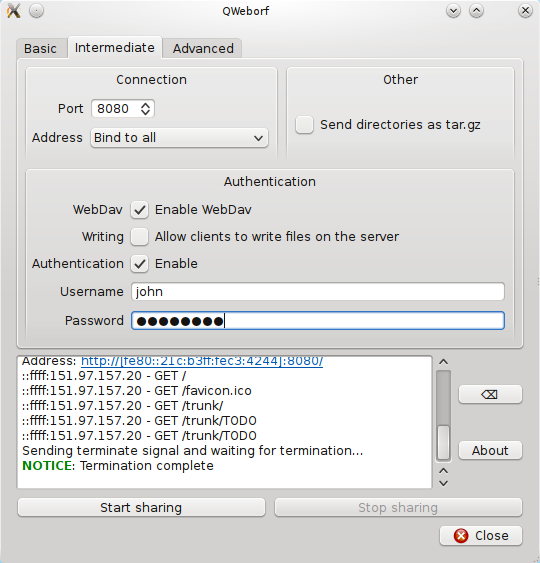
\includegraphics[width=7.655cm,height=7.98cm]{tesi-img1.png}
\captionof{figure}{qweborf, interfaccia di configurazione per utenti
avanzati}
\end{minipage} \begin{minipage}{7.655cm}
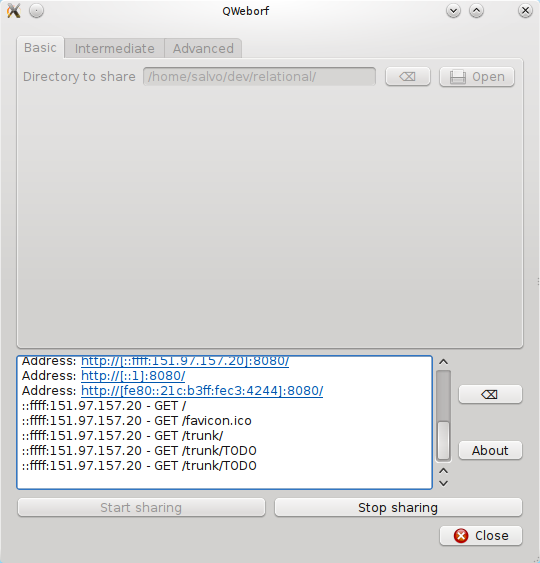
\includegraphics[width=7.655cm,height=7.98cm]{tesi-img2.png}
\captionof{figure}{qweborf, interfaccia semplice}
\end{minipage}}


\bigskip

{\sffamily
Iniziando la condivisione, nella parte inferiore della finestra appaiono
una serie di link cliccabili, che indicano i vari indirizzi IP su cui
il server sta ascoltando. Cliccando su uno degli indirizzi si aprir\`a
il browser predefinito dell{\textquotesingle}utente, che mostrer\`a la
pagina generata dal server weborf, contenente l{\textquotesingle}elenco
dei file.}

{\sffamily
Il secondo tab di configurazione presenta opzioni pi\`u avanzate:}

{\sffamily
\ \ {}- Opzioni di rete:}

{\sffamily
\ \ \ \ {}- Indirizzo IP su cui fare bind}

{\sffamily
\ \ \ \ \ \ Mostra l{\textquotesingle}elenco degli indirizzi IP della
macchina, e permette all{\textquotesingle}utente di sceglierne uno o di
accettare connessioni provenienti da tutti gli indirizzi IP.}

{\sffamily
\ \ \ \ {}- Porta}

{\sffamily
\ \ {}- Opzioni di autenticazione:}

{\sffamily
\ \ \ \ {}- Attivare webdav}

{\sffamily
\ \ \ \ \ \ Attiva i metodi PROPFIND e OPTIONS che servono per poter
utilizzare client DAV sulla condivisione}

{\sffamily
\ \ \ \ {}- Attivare scrittura}

{\sffamily
\ \ \ \ \ \ Attiva i metodi PUT,DELETE,COPY,MOVE,MKCOL che in maniera
differente permettono ciascuno di effettuare modifiche ai dati sul
server. Quando questa opzione \`e attivata, viene visualizzato un
warning nella parte inferiore dell{\textquotesingle}interfaccia, per
notificare possibili problemi di sicurezza dovuti a questa scelta.}

{\sffamily
\ \ \ \ {}- Username e password}

{\sffamily
\ \ \ \ \ \ Se inseriti, solo i client che forniscono queste
informazioni di login saranno autorizzati ad accedere.}

{\sffamily
\ \ {}- Altre opzioni}

{\sffamily
\ \ \ \ {}- Inviare le directory come .tar.gz}

{\sffamily
\ \ \ \ \ \ Attiva l{\textquotesingle}invio delle directory come file
.tar.gz invece che mostrare la lista dei file.}


\bigskip

{\sffamily
Il componente situato nella parte inferiore
dell{\textquotesingle}interfaccia (QTextBrowser) consente la
visualizzazione di testo semplice e di HTML. Questa caratteristica
viene utilizzata per visualizzare in colore diverso i vari messaggi per
l{\textquotesingle}utente e dare loro un impatto immediato differente.
Inoltre i link inseriti nel componente diventano automaticamente
cliccabili e vengono aperti nel browser predefinito.}

{\sffamily
Accanto, due pulsanti permettono di eliminare il log, e di mostrare le
informazioni relative al software all{\textquotesingle}interno della
stessa casella per i log.}


\bigskip

\subsection{Linguaggio e compatibilit\`a}
{\sffamily
Il linguaggio scelto per lo sviluppo dell{\textquotesingle}interfaccia
grafica \`e Python (versione 2), mentre il toolkit grafico usato \`e
Qt4. Viene utilizzata la libreria PyQt di Riverbanks per interfacciare
le librerie QT (scritte in C++) con il codice Python.}

{\sffamily
Sia Python che QT sono presenti sui maggiori sistemi operativi. Tuttavia
il modulo che ottiene gli indirizzi IP della macchina utilizza chiamate
di sistema specifiche Linux e quindi non \`e portabile. Ne segue che
attualmente l{\textquotesingle}intera interfaccia grafica non \`e
portabile ma sarebbe sufficiente effettuare il porting di quel singolo
modulo perch\'e l{\textquotesingle}intero programma possa essere
eseguito su altri sistemi.}


\bigskip

\subsection{Funzionamento}
{\sffamily
All{\textquotesingle}avvio l{\textquotesingle}interfaccia controlla la
presenza dell{\textquotesingle}eseguibile weborf
all{\textquotesingle}interno del PATH. Poi il programma weborf viene
eseguito con i parametri -v e -h per ottenere la versione e con quali
caratteristiche \`e stato compilato, ed eventualmente disattiva la
scelta di opzioni che non sono state compilate nel binario (ad esempio
se il binario \`e stato compilato senza il supporto per webdav).}

{\sffamily
Fino all{\textquotesingle}avvio del server, la gestione \`e unicamente
demandata al codice generato automaticamente dai tool di PyQt.}

{\sffamily
L{\textquotesingle}inizio della condivisione causa la creazione di una
unix socket che viene utilizzata dal server per richiedere
l{\textquotesingle}autorizzazione alle singole richieste. La socket
viene ascoltata da un thread di qweborf, che autorizza o nega le
richieste in base alla configurazione inserita prima di avviare la
condivisione. Inoltre un thread che si blocca su wait() che attende la
terminazione del processo weborf viene creato. Ed invia un evento al
resto del processo qualora il server dovesse terminare.}


\bigskip

{\sffamily
Il thread che garantisce o nega l{\textquotesingle}autorizzazione alle
singole richieste, riceve tutti i dettagli sulle connessioni in arrivo,
e tali dettagli vengono visualizzati nella parte inferiore
dell{\textquotesingle}interfaccia grafica.}


\bigskip

{\sffamily
I vari thread comunicano tra loro passandosi oggetti utilizzando le
primitive QT per emit() e connect(), in modo da evitare problemi di
sincronizzazione, che potrebbero anche causare una terminazione con
errore\cite{QT01}.}


\bigskip

{\sffamily
La terminazione della condivisione causa l{\textquotesingle}invio di un
segnale SIGINT al server weborf, e la generazione di un evento
all{\textquotesingle}interno di qweborf quando il processo figlio
termina effettivamente la sua esecuzione. Vengono mostrate due entry
nel log, per indicare l{\textquotesingle}invio del segnale e
l{\textquotesingle}avvenuta terminazione del server.}


\bigskip

\subsection{Integrazione desktop}
{\sffamily
Un file .desktop viene distribuito assieme al codice, per mostrare una
voce nel menu del desktop.}

{\sffamily
Una pagina di manuale viene distribuita, per indicare principalmente lo
scopo del programma, dato che non dispone di alcuno switch da linea di
comando.}


\bigskip

\section{Demone}
{\sffamily
Per poter essere eseguito come demone SystemV weborf include uno script
di avvio.}


\bigskip

{\sffamily
Tale script si occupa di leggere il file di configurazione situato in
/etc/weborf.conf e di eseguire il comando weborf con la appropriata
riga di comando (a causa del fatto che l{\textquotesingle}eseguibile in
se non ha nessun modo di caricare file di configurazione).}


\bigskip

{\sffamily
Per evitare che vengano eseguite pi\`u istanze di weborf con la stessa
configurazione, lo script demone salva il pid del processo weborf in
/var/run/weborf.pid, permettendo anche di poter recuperare il processo
e terminarlo quando venisse richiesto.}


\bigskip

{\sffamily
Oltre ai consueti parametri {\textquotedbl}start{\textquotedbl} e
{\textquotedbl}stop{\textquotedbl}, sono presenti anche
{\textquotedbl}force-reload{\textquotedbl},
{\textquotedbl}restart{\textquotedbl} e
{\textquotedbl}status{\textquotedbl} che indica se il server \`e in
esecuzione o meno.}

{\sffamily
Bisogna notare che qualora il comando status dicesse che il server non
\`e in esecuzione, questo non implicherebbe che non vi siano processi
weborf in esecuzione attualmente, ma solo che essi non sono stati
lanciati come demone.}


\bigskip

\subsection{Linux Standard Base}
{\sffamily
Linux Standard Base (LSB) \`e uno standard che tenta di unificare le
varie distribuzioni. Lo script per usare weborf come demone rispetta
correttamente lo standard (\`e stato controllato da lintian),
includendo il supporto a tutti i parametri richiesti, e la
possibilit\`a di usare un dependency based boot.}


\bigskip

{\sffamily
Il dependency based boot consente di modificare
l{\textquotesingle}ordine di avvio dei vari servizi in base alle
interdipendenze che hanno i vari servizi gli uni dagli altri. Per
ottenere questo risultato, ciascuno degli script di avvio di un
servizio deve contenere una sezione commentata che descrive le
dipendenze del servizio.}

{\sffamily
In tal modo si permette al tool specifico della distribuzione di poter
generare un grafo delle dipendenze e poter scegliere in maniera
automatica l{\textquotesingle}ordine di avvio migliore, numerando gli
script nelle directory /etc/rc come consueto\cite{LSB01}.}


\bigskip

{\sffamily
La sezione commentata nel demone appare cos\`i:}


\bigskip

{\ttfamily
\#\#\# BEGIN INIT INFO}

{\ttfamily
\# Provides: \ \ \ \ \ \ \ \ \ weborf}

{\ttfamily
\# Required-Start: \ \ \ \$network \$local\_fs \$syslog \$remote\_fs}

{\ttfamily
\# Required-Stop: \ \ \ \ \$remote\_fs}

{\ttfamily
\# Should-Start: \ \ \ \ \ \$named}

{\ttfamily
\# Should-Stop:}

{\ttfamily
\# Default-Start: \ \ \ \ 2 3 4 5}

{\ttfamily
\# Default-Stop: \ \ \ \ \ 0 1 6}

{\ttfamily
\# Short-Description: Fast and small webserver}

{\ttfamily
\# Description: \ \ \ \ \ \ Weborf is a configurationless webserver}

{\ttfamily
\# \ \ \ \ \ \ \ \ \ \ \ \ \ \ \ \ \ \ \ mainly meant to allow users}

{\ttfamily
\# \ \ \ \ \ \ \ \ \ \ \ \ \ \ \ \ \ \ \ to easily share their
directories over the}

{\ttfamily
\# \ \ \ \ \ \ \ \ \ \ \ \ \ \ \ \ \ \ \ web.}

{\ttfamily
\# \ \ \ \ \ \ \ \ \ \ \ \ \ \ \ \ \ \ \ It also supports php5-cgi.}

{\ttfamily
\#\#\# END INIT INFO}


\bigskip

{\sffamily
I nomi che iniziano con \$ sono dei placeholder per il servizio
effettivo che fornisce quel tipo di servizio. Ad esempio \$syslog pu\`o
venire soddisfatto da rsyslog e da syslogd\cite{LSB03}.}

{\sffamily
Quindi si evidenzia come vengano richiesti i servizi di rete, i
filesystem locali e remoti ed il sistema di log prima di poter avviare
il server weborf.}

{\sffamily
Tali informazioni hanno effetto solo quando si ordina
l{\textquotesingle}avvio dei servizi (su Debian questo avviene
lanciando il tool update-rc.d), non se si avvia un servizio manualmente
(infatti per bash sono semplicemente dei commenti).}

{\sffamily
Vengono anche forniti i runlevel in cui il servizio dovrebbe partire e
quelli in cui dovrebbe fermarsi.}


\bigskip

\section{Debian packaging}
{\sffamily
L{\textquotesingle}intero progetto \`e presente
all{\textquotesingle}interno della distribuzione Debian\cite{LSB04}. E viene
automaticamente importato in maniera periodica da Ubuntu,
all{\textquotesingle}interno dei loro repository universe.}


\bigskip

{\sffamily
Per creare un pacchetto .deb in maniera corretta si deve creare tramite
{\textquotedbl}make dist{\textquotedbl} il tar.gz del progetto,
rinominarlo perch\'e soddisfi le convenzioni usate da debian e poi
estrarne il contenuto, che si utilizzer\`a per la creazione del
pacchetto. Si creer\`a una directory
{\textquotedbl}debian/{\textquotedbl} all{\textquotesingle}interno
della directory contenente i sorgenti.}


\bigskip

{\sffamily
All{\textquotesingle}interno della directory debian si \`e proceduto
alla creazione del file di make {\textquotedbl}rules{\textquotedbl},
indicando essenzialmente di eseguire il makefile di weborf e di copiare
i file python di qweborf nelle relative locazioni corrette.}

{\sffamily
Il file control contiene l{\textquotesingle}elenco dei pacchetti binari
da creare, con le relative descrizioni e dipendenze, e le dipendenze
necessarie alla compilazione.}


\bigskip

{\sffamily
I tool dpkg vengono utilizzati per creare i file di patch da applicare
all{\textquotesingle}archivio originario, per compilare e creare i
pacchetti deb.}

{\sffamily
Lintian \`e stato utilizzato per verificare la correttezza dei
pacchetti. Ha consentito di individuare alcuni errori nella
formattazione delle pagine di manuale distribuite con i binari.}


\bigskip

{\sffamily
Per regole di Debian, la directory debian/ non pu\`o essere distribuita
assieme al sorgente ma deve essere inclusa separatamente sotto forma di
patch.}


\bigskip

{\sffamily
La versione del pacchetto deve essere impostata tramite il comando
{\textquotedbl}dch{\textquotedbl}, che aggiunge una voce al changelog
del pacchetto, che le policy di Debian impongono di distribuire.}


\bigskip

\section[Comparazione prestazioni]{Comparazione prestazioni}
{\sffamily
Comparare le prestazioni non \`e un lavoro facile. Si rischia di
evidenziare comportamenti che si presentano solo in una specifica
condizione ma che sono assolutamente irrilevanti con tipi di carico
misto.}


\bigskip

{\sffamily
Per evitare di ottenere risultati falsati, ed avere risultati il pi\`u
possibile attinenti alla realt\`a, si utilizzano diversi carichi di
lavoro sia statici che dinamici in modo da ottenere una rilevazione dei
diversi comportamenti nelle varie situazioni. Per i tipi di carico in
cui \`e possibile utilizzare il sistema di caching implementato in
weborf, sono stati effettuati test in maniera duplicata per evidenziare
la differenza di comportamento con o senza caching.}


\bigskip

{\sffamily
Leggendo i test si dovr\`a tenere conto della natura del test stesso e
considerare che il caso reale \`e pi\`u simile ad una mescolanza dei
differenti tipi di carico.}


\bigskip

\subsection{Tool di benchmark}
{\sffamily
Viene utilizzato il tool apache benchmark che fa parte della suite
Apache per effettuare i test. Gravei limitazioni di tale tool sono
l{\textquotesingle}impossibilit\`a ad utilizzarlo per tutti i metodi
HTTP in maniera generalizzata, e il mancato supporto a WEBDAV.}

{\sffamily
Questo tool effettua la stessa richiesta in maniera ripetuta verso il
server, quindi non dando alcuna informazione sul comportamento del
server con i carichi misti.}

{\sffamily
Per mitigare il problema sono stati effettuati diversi tipi di test con
diversi tipi di contenuto e parallelismo, in modo da ottenere una idea
pi\`u globale della situazione.}

{\sffamily
\`E necessario tenere in conto che il kernel Linux non \`e real-time e
questo pu\`o generare anche notevoli variazioni nei risultati di uno
stesso test, eseguito sulla stessa macchina, apparentemente con le
stesse identiche condizioni.}


\bigskip

\subsection[Sistema di test]{Sistema di test}
{\sffamily
Il sistema utilizzato per i test comprende un disco SATA che utilizza
filesystem reiserfs, una CPU Intel(R) Core(TM)2 CPU T7200 \ @ 2.00GHz
ed esegue un kernel Linux 2.6.38.6 ed una eglibc 2.13.}

{\sffamily
Il sistema utilizzato \`e a 64 bit.}

{\sffamily
Per evitare di misurare le prestazioni della rete invece che quelle dei
server web, tutti i test sono stati effettuati utilizzando
l{\textquotesingle}interfaccia virtuale di loopback invece che delle
reali interfacce di rete.}


\bigskip

\subsection{Versioni usate}
\begin{flushleft}
\bottomcaption{Versioni di server web utilizzate per i test.}
\tablehead{}
\begin{supertabular}{|m{4.2450004cm}|m{5.4620004cm}|}
\hline
\sffamily weborf &
\sffamily 0.13-1\\\hline
\sffamily lighttpd &
\sffamily 1.4.28-5\\\hline
\sffamily nginx &
\sffamily 1.0.1-1\\\hline
\sffamily apache &
\sffamily 2.2.19-1\\\hline
\end{supertabular}
\end{flushleft}
{\sffamily
Tutte le versioni sono state installate dai repository debian, e
compilate con le stesse opzioni e la stessa versione di compilatore.}


\bigskip

\subsection{Risultati dei test}
{\sffamily
Ogni test \`e stato effettuato diverse volte, variando il parallelismo
utilizzato.}

{\sffamily
Sono stati effettuati test per ciascun tipo di carico utilizzando 1
thread soltanto, 20, 50, 100 e 200. In tal modo si \`e inteso ottenere
risultati sul comportamento del server al variare del carico totale.}

{\sffamily
In quasi tutti i test si nota che il server non riesce a raggiungere la
piena velocit\`a quando viene effettuata una sola richiesta per volta.}


\bigskip

{\sffamily
Nei grafici di seguito presentati, i valori sulle ascisse rappresentano
il livello di parallelismo, mentre quelli sulle ordinate indicano il
numero di richieste al secondo che il server riesce a soddisfare per
quel particolare tipo di carico.}

\begin{minipage}{16cm}
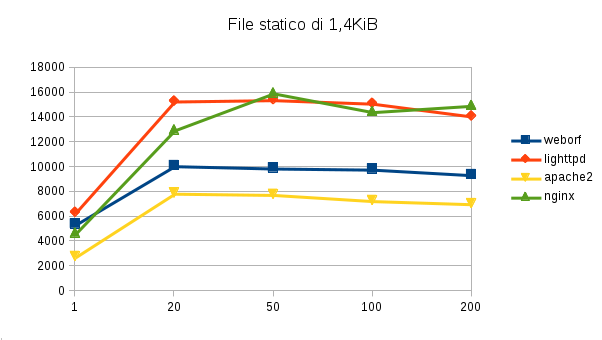
\includegraphics[width=16cm,height=8.999cm]{tesi-img3.png}
\captionof{figure}{Comparazione velocit\`a sull{\textquotesingle}invio
di file statico della dimensione di 1,4KiB}
\end{minipage}

{\sffamily
In questo test si \`e provato a richiedere ai server di inviare un
piccolo file statico. Questo tipo di carico \`e molto comune perch\'e
la maggior parte dei siti web si compone di file molto piccoli come CSS
o HTML.}


\bigskip

\begin{minipage}{16cm}
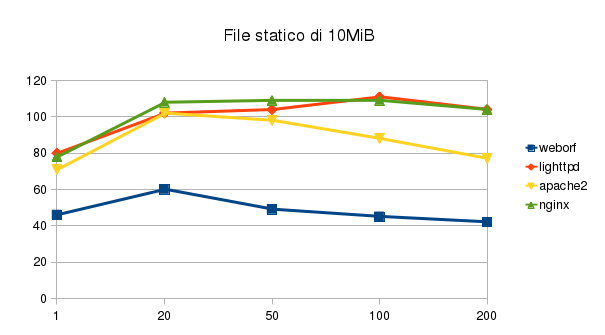
\includegraphics[width=16cm,height=8.999cm]{tesi-img4.png}
\captionof{figure}{Comparazione velocit\`a sull{\textquotesingle}invio
di file statico della dimensione di 10MiB}
\end{minipage}

{\sffamily
In questo test si \`e provato invece a valutare il comportamento quando
il file statico richiesto \`e di dimensioni pi\`u grandi.}

\begin{minipage}{16cm}
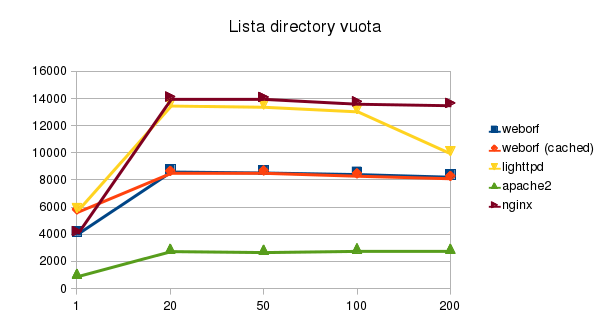
\includegraphics[width=15.998cm,height=8.999cm]{tesi-img5.png}
\captionof{figure}{Comparazione velocit\`a sull{\textquotesingle}invio
di una lista di files contenuti in una directory vuota.}
\end{minipage}

{\sffamily
In questo test si \`e chiesto ai server di generare dinamicamente una
lista in formato HTML.}

{\sffamily
Per weborf i test sono stati effettuati due volte, per differenziare tra
l{\textquotesingle}utilizzo della cache ed il mancato utilizzo. Si nota
una sostanziale equivalenza nei due casi.}


\bigskip

\begin{minipage}{16cm}
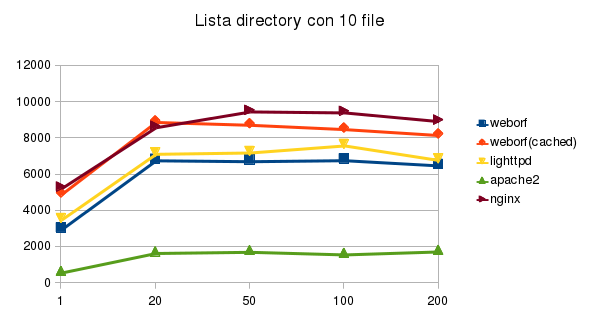
\includegraphics[width=16cm,height=8.999cm]{tesi-img6.png}
\captionof{figure}{Comparazione velocit\`a sull{\textquotesingle}invio
di una lista di files contenuti in una directory con 10 file.}
\end{minipage}

{\sffamily
In questo test invece si \`e utilizzata una directory contenente 10
file, in modo da rendere per il server pi\`u onerosa
l{\textquotesingle}operazione di creazione della lista dei file in
formato HTML. Si nota qui che la versione con cache di weborf \`e pi\`u
veloce della versione senza cache, ma comunque pi\`u lenta di nginx.}


\bigskip

\begin{minipage}{16cm}
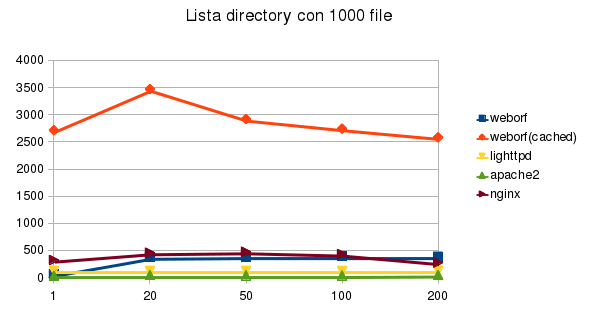
\includegraphics[width=16cm,height=8.999cm]{tesi-img7.png}
\captionof{figure}{Comparazione velocit\`a sull{\textquotesingle}invio
di una lista di files contenuti in una directory con 1000 file.}
\end{minipage}

{\sffamily
Per questo test si \`e utilizzata una directory contenente 1000 file, in
modo da rendere estremamente onerosa la gestione della richiesta.}

{\sffamily
Qui si nota in maniera evidente il vantaggio di utilizzare una cache
rispetto alla soluzione di generare dinamicamente la lista ad ogni
richiesta da parte di un client.}


\bigskip

\begin{minipage}{16cm}
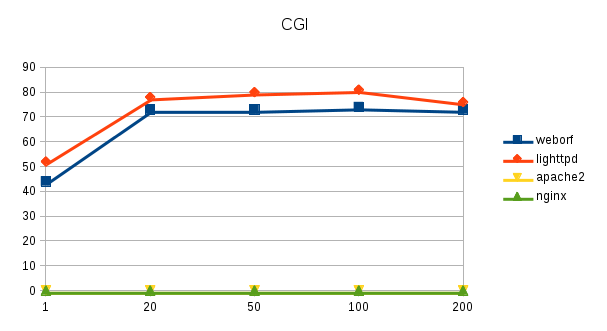
\includegraphics[width=16cm,height=8.999cm]{tesi-img8.png}
\captionof{figure}{Comparazione performances di una semplice pagina php
che chiama la funzione phpinfo() utilizzata tramite protocollo CGI.
Nginx non supporta CGI, apache2 non supporta
l{\textquotesingle}utilizzo di php tramite CGI.}
\end{minipage}

{\sffamily
Questo test confronta l{\textquotesingle}esecuzione di script CGI.}


\bigskip

\section{Glossario}
{\sffamily
Contenuto dinamico: Un contenuto dinamico viene generato da un programma
quando viene ricevuta una certa richiesta.}


\bigskip

{\sffamily
Contenuto statico: Un contenuto statico \`e contenuto in un file su
disco e viene inviato al client quando viene ricevuta una certa
richiesta.}


\bigskip

{\sffamily
File grandi: Per file grandi si intendono file che hanno una dimensione
superiore a 2{\textthreesuperior}{\texttwosuperior}, che quindi non
pu\`o essere contenuta in variabili intere senza segno a 32 bit.}


\bigskip

{\sffamily
Keep-Alive: \`E un meccanismo introdotto nel protocollo HTTP a partire
dalla versione 1.0, e reso default nella versione 1.1. Consente
l{\textquotesingle}invio di pi\`u richieste
all{\textquotesingle}interno della stessa connessione. Ogni richiesta
viene terminata dalla sequenza
{\textquotedbl}{\textbackslash}r{\textbackslash}n{\textbackslash}r{\textbackslash}n{\textquotedbl}
e pu\`o essere seguita da un{\textquotesingle}altra richiesta oppure da
dati grezzi. Nel secondo caso nella richiesta stessa deve essere
indicata la dimensione in byte dei dati grezzi allegati alla
richiesta.}

{\sffamily
Le risposte contengono un header terminato da
{\textquotedbl}{\textbackslash}r{\textbackslash}n{\textbackslash}r{\textbackslash}n{\textquotedbl}
e sono seguite da dati grezzi la cui lunghezza deve essere specificata
all{\textquotesingle}interno dell{\textquotesingle}header stesso. Nel
caso in cui sia impossibile conoscere a priori la dimensione dei dati
che si stanno per inviare, si utilizza la chiusura della connessione
come marcatore.}


\bigskip

\section{Conclusioni}
\subsection{Reazioni degli utenti}
{\sffamily
Il numero pubblicato a Giugno 2011 di Linux Magazin in Germania riporta
un breve articolo su weborf\cite{LNK01}.}

{\sffamily
La distribuzione GNU/Linux tedesca per dispositivi embedded Freetz
fornisce un pacchetto per weborf, e commenti indicano sia apprezzato
per le piccole dimensioni\cite{LNK02}.}

{\sffamily
Alcuni blog e forum ne consigliano
l{\textquotesingle}utilizzo\cite{LNK03}\cite{LNK04}.}

{\sffamily
I contatori di download sono poco informativi in quanto non forniscono
nessuna reale informazione riguardante il numero di utenti effettivi.}

{\sffamily
In generale \`e impossibile conoscere il numero di utenti, ad ogni modo
il popularity contest di Ubuntu indica:}

\begin{center}
\bottomcaption{Installazioni su sistemi Ubuntu che partecipano al
popularity contest.}
\tablehead{}
\begin{supertabular}{|m{8.3cm}|m{8.3cm}|}
\hline
\sffamily weborf &
\sffamily 77\\\hline
\sffamily weborf-daemon &
\sffamily 29\\\hline
\end{supertabular}
\end{center}
{\sffamily
Mentre il popularity contest di Debian fornisce un dato pi\`u accurato
mostrando l{\textquotesingle}andamento nel tempo.}

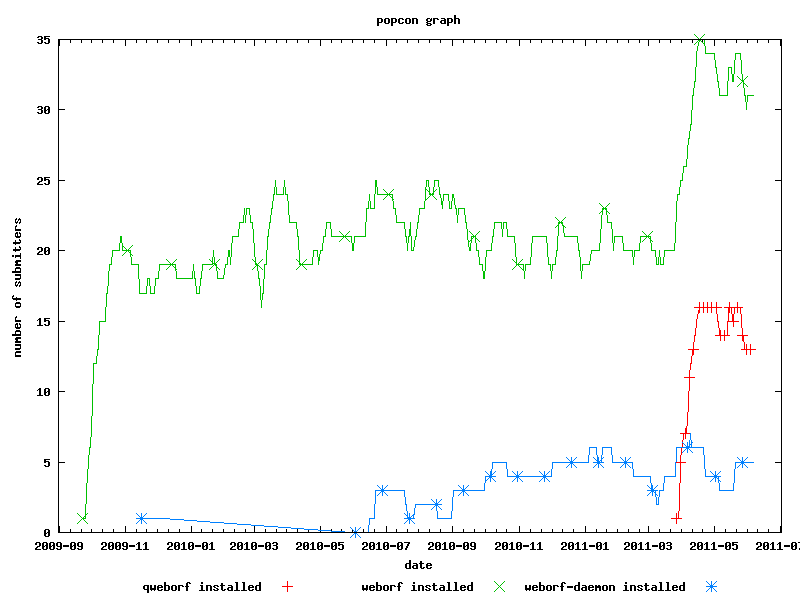
\includegraphics[width=17cm,height=12.749cm]{tesi-img9.png}
\captionof{figure}[Installazioni di weborf sui sistemi debian che
partecipano al popularity contest.]{Installazioni di weborf sui sistemi
debian che partecipano al popularity contest.}


\subsection{Sviluppi futuri}
{\sffamily
La tecnologia della cache per i contenuti generati dal server \`e
particolarmente interessante e sarebbe auspicabile implementarla
all{\textquotesingle}interno di un modulo per dei web server pi\`u
famosi e pi\`u supportati, e che gi\`a dispongono di numerose
estensioni; il server migliore su cui implementare tale modulo sarebbe
Apache2.}

{\sffamily
Ridurre ulteriormente il memory footprint sia su RAM che su disco \`e un
altro obiettivo auspicabile per l{\textquotesingle}utilizzo sui sistemi
embedded.}

{\sffamily
Utilizzare SSL nelle prossime versioni \`e uno degli obiettivi. Si
richiederebbe anche la scrittura di una libreria per incapsulare le
letture e le scritture da parte di processi figli che attualmente
scrivono direttamente sul descrittore di file (come nel caso
dell{\textquotesingle}invio di directory compresse utilizzando
.tar.gz), in modo tale che le letture e scritture sul descrittore di
file vengano incapsulate e sia fornito un layer che fornisca cifratura
ed autenticazione in maniera trasparente per i processi figli.}

\section{Bibliografia}

% \section{References}
% (Re-use from previous documents, extend.)
\bibliographystyle{plainnat}
\bibliography{refs}

\bigskip

\section[Ringraziamenti]{\sffamily Ringraziamenti}
{\sffamily
Il relatore prof. Giuseppe Pappalardo.}

{\sffamily
Sandun Fernando per le numerose prove effettuate.}

{\sffamily
Salvo Rinaldi per gli stimoli forniti.}

{\sffamily
Milena Aliberti per le prove di usabilit\`a di qweborf.}

{\sffamily
David Paleino ed Enrico Zini per consigli su come creare i pacchetti
Debian}

{\sffamily
David Kalnischkies per i suggerimenti su come aumentare
l{\textquotesingle}aderenza al protocollo HTTP.}

\section[Appendice A]{Appendice A}
{\sffamily
Per comparare la velocit\`a della chiamata di sistema sendfile() con
l{\textquotesingle}approccio pi\`u comune di utilizzare chiamate read()
e write() si \`e creato un programma di esempio.}

{\sffamily
Tale programma accetta connessioni su una socket IPv4, apre un file e
copia l{\textquotesingle}intero file sulla socket.}


\bigskip

{\sffamily
Per misurare la velocit\`a si \`e usato questo comando:}

{\ttfamily
time nc localhost 12345 {\textgreater} /dev/null}


\bigskip

{\sffamily
Il programma \`e stato compilato ed eseguito alternativamente usando la
funzione fd\_copy e la chiamata di sistema sendfile().}

{\sffamily
Il file test.dat utilizzato era grande circa 670MiB e conteneva dati
generati casualmente utilizzando il comando:}

{\sffamily
cat /dev/urandom {\textgreater} test.dat}

{\sffamily
dato che un file enorme generato con truncate avrebbe probabilmente
generato risultati falsati.}


\bigskip

{\sffamily
Segue il sorgente del programma di prova:}

{\ttfamily
\#include {\textless}arpa/inet.h{\textgreater}}

{\ttfamily
\#include {\textless}sys/types.h{\textgreater}}

{\ttfamily
\#include {\textless}sys/stat.h{\textgreater}}

{\ttfamily
\#include {\textless}sys/socket.h{\textgreater}}

{\ttfamily
\#include {\textless}sys/sendfile.h{\textgreater}}

{\ttfamily
\#include {\textless}stdio.h{\textgreater}}

{\ttfamily
\#include {\textless}string.h{\textgreater}}

{\ttfamily
\#include {\textless}fcntl.h{\textgreater}}

{\ttfamily
\#include {\textless}stdlib.h{\textgreater}}

{\ttfamily
\#include {\textless}unistd.h{\textgreater}}


\bigskip

{\ttfamily
\#define FILEBUF 4096}


\bigskip

{\ttfamily
typedef struct \{}

{\ttfamily
\ \ \ \ int fd;}

{\ttfamily
\ \ \ \ size\_t size;}

{\ttfamily
\} file\_t;}


\bigskip

{\ttfamily
int fd\_copy(int from, int to, off\_t count) \{}

{\ttfamily
\ \ \ \ char *buf=malloc(FILEBUF);//Buffer to read from file}

{\ttfamily
\ \ \ \ int reads,wrote;}

{\ttfamily
\ \ \ \ int retval=0;}


\bigskip

{\ttfamily
\ \ \ \ //Sends file}

{\ttfamily
\ \ \ \ while (count{\textgreater}0 \&\& (reads=read(from, buf,
FILEBUF{\textless}count? FILEBUF:count )){\textgreater}0) \{}

{\ttfamily
\ \ \ \ \ \ \ \ count-=reads;}

{\ttfamily
\ \ \ \ \ \ \ \ wrote=write(to,buf,reads);}

{\ttfamily
\ \ \ \ \ \ \ \ if (wrote!=reads) \{ //Error writing to the descriptor}

{\ttfamily
\ \ \ \ \ \ \ \ \ \ \ \ retval=1;}

{\ttfamily
\ \ \ \ \ \ \ \ \ \ \ \ break;}

{\ttfamily
\ \ \ \ \ \ \ \ \}}

{\ttfamily
\ \ \ \ \}}


\bigskip

{\ttfamily
\ \ \ \ free(buf);}

{\ttfamily
\ \ \ \ return retval;}

{\ttfamily
\}}


\bigskip

{\ttfamily
int acceptsocket(int port) \{}

{\ttfamily
\ \ \ \ int sockfd, newsockfd;}

{\ttfamily
\ \ \ \ socklen\_t clilen;}

{\ttfamily
\ \ \ \ struct sockaddr\_in serv\_addr, cli\_addr;}


\bigskip

{\ttfamily
\ \ \ \ sockfd = socket(AF\_INET, SOCK\_STREAM, 0);}

{\ttfamily
\ \ \ \ bzero((char *) \&serv\_addr, sizeof(serv\_addr));}


\bigskip

{\ttfamily
\ \ \ \ serv\_addr.sin\_family = AF\_INET;}

{\ttfamily
\ \ \ \ serv\_addr.sin\_addr.s\_addr = INADDR\_ANY;}

{\ttfamily
\ \ \ \ serv\_addr.sin\_port = htons(port);}

{\ttfamily
\ \ \ \ \{}

{\ttfamily
\ \ \ \ \ \ \ \ int val=1;}

{\ttfamily
\ \ \ \ \ \ \ \ setsockopt(sockfd, SOL\_SOCKET, SO\_REUSEADDR, \&val,
sizeof(val));}

{\ttfamily
\ \ \ \ \}}

{\ttfamily
\ \ \ \ if (bind(sockfd, (struct sockaddr *) \&serv\_addr,}

{\ttfamily
\ \ \ \ \ \ \ \ \ \ \ \ \ sizeof(serv\_addr)) {\textless} 0)}

{\ttfamily
\ \ \ \ \ \ \ \ error({\textquotedbl}ERROR on binding{\textquotedbl});}

{\ttfamily
\ \ \ \ listen(sockfd,5);}

{\ttfamily
\ \ \ \ clilen = sizeof(cli\_addr);}

{\ttfamily
\ \ \ \ newsockfd = accept(sockfd,NULL,NULL);}

{\ttfamily
\ \ \ \ if (newsockfd {\textless} 0)}

{\ttfamily
\ \ \ \ \ \ \ \ error({\textquotedbl}ERROR on accept{\textquotedbl});}

{\ttfamily
\ \ \ \ return newsockfd;}

{\ttfamily
\}}


\bigskip

{\ttfamily
file\_t openfile(char *fname) \{}

{\ttfamily
\ \ \ \ file\_t r;}

{\ttfamily
\ \ \ \ struct stat buf;}


\bigskip

{\ttfamily
\ \ \ \ r.fd=open(fname,O\_RDONLY);}


\bigskip

{\ttfamily
\ \ \ \ fstat(r.fd,\&buf);}


\bigskip

{\ttfamily
\ \ \ \ r.size=buf.st\_size;}

{\ttfamily
\ \ \ \ return r;}

{\ttfamily
\}}


\bigskip

{\ttfamily
int main () \{}

{\ttfamily
\ \ \ \ file\_t
locfile=openfile({\textquotedbl}/tmp/test.dat{\textquotedbl});}

{\ttfamily
\ \ \ \ int sock=acceptsocket(12345);}


\bigskip

{\ttfamily
\ \ \ \ printf({\textquotedbl}file fd: \%d{\textbackslash}nsocket fd:
\%d{\textbackslash}n{\textquotedbl},locfile.fd,sock);}

{\ttfamily
\ \ \ \ //sendfile(sock, locfile.fd, NULL,locfile.size);}

{\ttfamily
\ \ \ \ fd\_copy(locfile.fd,sock,locfile.size);}

{\ttfamily
\ \ \ \ return 0;}

{\ttfamily
\}}

\subsection{Risultati}
{\sffamily
Ciascuna modalit\`a \`e stata testata tre volte sullo stesso file, i
risultati di media sono i seguenti:}

\begin{flushleft}
\bottomcaption{Comparazione risultati del codice di prova, utilizzando
sendfile oppure no.}
\tablehead{}
\begin{supertabular}{|m{3.291cm}|m{5.859cm}|}
\hline
\sffamily sendfile &
\sffamily 24.164s\\\hline
\sffamily fd\_copy &
\sffamily 21.422s\\\hline
\end{supertabular}
\end{flushleft}
\end{document}
